%%%%%%%%%%%%%%%%%%%%%%%%%%%%%%%%%%%%%%%%%%%%%%%%%%%%%%%%%%%%%%%%%
% MUW Presentation
% LaTeX Template
% Version 1.0 (27/12/2016)
%
% License:
% CC BY-NC-SA 4.0 (http://creativecommons.org/licenses/by-nc-sa/3.0/)
%
% Created by:
% Nicolas Ballarini, CeMSIIS, Medical University of Vienna
% nicoballarini@gmail.com
% http://statistics.msi.meduniwien.ac.at/
%
% Customized for UAH by:
% David F. Barrero, Departamento de Automática, UAH
%%%%%%%%%%%%%%%%%%%%%%%%%%%%%%%%%%%%%%%%%%%%%%%%%%%%%%%%%%%%%%%%%

\documentclass[10pt,compress]{beamer} % Change 10pt to make fonts of a different size
\mode<presentation>

\usepackage[spanish]{babel}
\usepackage{fontspec}
\usepackage{tikz}
\usepackage{etoolbox}
\usepackage{xcolor}
\usepackage{xstring}
\usepackage{listings}
\usepackage{multicol}

% Custom packages
\usepackage{algpseudocode}
\usepackage{tikz}
\usepackage{pgfplots}
\def\layersep{2.5cm}
\usetikzlibrary{matrix,chains,positioning,decorations.pathreplacing,arrows}

\definecolor{dkgreen}{rgb}{0,0.6,0}
\definecolor{gray}{rgb}{0.5,0.5,0.5}
\definecolor{mauve}{rgb}{0.58,0,0.82}
 

\usetheme{UAH}
\usecolortheme{UAH}
\setbeamertemplate{navigation symbols}{} 
\setbeamertemplate{caption}[numbered]

%%%%%%%%%%%%%%%%%%%%%%%%%%%%%%%%%%%%%%%%%%%%%%%%%%%%%%%%%%%%%%%%%
%% Presentation Info
\title[Aritificial Neural Networks]{Artificial Neural Networks}
\author{\asignatura\\\carrera}
\institute{}
\date{Departamento de Automática}
%%%%%%%%%%%%%%%%%%%%%%%%%%%%%%%%%%%%%%%%%%%%%%%%%%%%%%%%%%%%%%%%%


%%%%%%%%%%%%%%%%%%%%%%%%%%%%%%%%%%%%%%%%%%%%%%%%%%%%%%%%%%%%%%%%%
%% Descomentar para habilitar barra de navegación superior
\setNavigation
%%%%%%%%%%%%%%%%%%%%%%%%%%%%%%%%%%%%%%%%%%%%%%%%%%%%%%%%%%%%%%%%%

%%%%%%%%%%%%%%%%%%%%%%%%%%%%%%%%%%%%%%%%%%%%%%%%%%%%%%%%%%%%%%%%%
%% Configuración de logotipos en portada
%% Opacidad de los logotipos
\newcommand{\opacidad}{1}
%% Descomentar para habilitar logotipo en pié de página de portada
\renewcommand{\logoUno}{Images/isg.png}
%% Descomentar para habilitar logotipo en pié de página de portada
%\renewcommand{\logoDos}{Images/CCLogo.png}
%% Descomentar para habilitar logotipo en pié de página de portada
%\renewcommand{\logoTres}{Images/ALogo.png}
%% Descomentar para habilitar logotipo en pié de página de portada
%\renewcommand{\logoCuatro}{Images/ELogo.png}
%%%%%%%%%%%%%%%%%%%%%%%%%%%%%%%%%%%%%%%%%%%%%%%%%%%%%%%%%%%%%%%%%

%%%%%%%%%%%%%%%%%%%%%%%%%%%%%%%%%%%%%%%%%%%%%%%%%%%%%%%%%%%%%%%%%
%% FOOTLINE
%% Comment/Uncomment the following blocks to modify the footline
%% content in the body slides. 


%% Option A: Title and institute
\footlineA
%% Option B: Author and institute
%\footlineB
%% Option C: Title, Author and institute
%\footlineC
%%%%%%%%%%%%%%%%%%%%%%%%%%%%%%%%%%%%%%%%%%%%%%%%%%%%%%%%%%%%%%%%%

\begin{document}

%%%%%%%%%%%%%%%%%%%%%%%%%%%%%%%%%%%%%%%%%%%%%%%%%%%%%%%%%%%%%%%%%
% Use this block for a blue title slide with modified footline
{\titlepageBlue
    \begin{frame}
        \titlepage
    \end{frame}
}

\institute{\asignatura}

\begin{frame}[plain]{}
   \begin{block}{Objectives}
      \begin{enumerate}
         \item Describe biological neurons and networks
         \item Basics of artifical neurons and networks
         \item Understand the role of trainning in ANNs
         \item Strengths and weaknesses of ANNs
      \end{enumerate} 
   \end{block}

   \begin{block}{Bibliography}
	\begin{itemize}
        \item A. Tettamanzi, M. Tomassini. \textit{Soft Computing. Integrating Evolutionary, Neural, and Fuzzy Systems}. Springer-Verlag. 2001
	    \item McCulloch, W. and Pitts, W. (1943). \textit{A logical calculus of the ideas immanent in nervous activity}. Bulletin of Mathematical Biophysics, 7:115 - 133. 
	    \item Rosenblatt, Frank.  (1958). \textit{The Perceptron: A Probabilistic Model for Information Storage and Organization in the Brain}. Psychological Review, 65:386-408
	\end{itemize}
   \end{block}
\end{frame}

{
\disableNavigation{white}
\begin{frame}[shrink]{Table of Contents}
 \frametitle{Table of Contents}

    \begin{multicols}{2}
    \tableofcontents
    \end{multicols}
  % You might wish to add the option [pausesections]
\end{frame}
}

\section{Introduction}

%\subsection{Machine Learning tasks}
%\begin{frame}{Introduction}{Machine Learning (I)}
%	Machine Learning studies how to build data-driven models
%	\begin{itemize}
%	\item \textbf{Supervised learning} The dataset contains output examples
%	\begin{flushleft}
%		\begin{itemize}
%		\item \textbf{Classification} The output is a category
%		\item \textbf{Regression} The output is a number
%		\end{itemize}
%		\end{flushleft}
%	\item \textbf{Unsupervised learning} (or \textit{clustering}) The dataset does not contain output examples
%	\item \textbf{Reinforcement learning} Maximize reward
%	\end{itemize}
%	ML is data-driven
%\end{frame}

%\begin{frame}[plain]{Introduction}{Machine Learning (II)}
%	\note{Comparar data-driven con programacion clasica}
%	\begin{center}
%	\vspace{-0.3cm}
%		\includegraphics[width=0.44\linewidth]{figs/lifecycle.png}
%	\end{center}
%\end{frame}


\subsection{History}
\begin{frame}{Introduction}{History}
    \begin{columns}
 	   \column{.80\textwidth}

	\begin{itemize}
	\item[1888] \textit{Ramón y Cajal}. Discovery of biological neurons
	\item[1943] \textit{McCulloch \& Pitts}. First neural network designers
	\item[1949] \textit{Hebb}. First learning rule
	\item[1958] \textit{Rosenblatt}. Perceptron
	\item[1969] \textit{Minsky \& Papert}.  Perceptron limitation - Death of ANN
	\note{Single layer perceonptrons cannot represent (learn) simple functions such as XOR
	Multi-layer of non-linear units may have greater power but there is no learning rule for such nets
	Scaling problem: connection weights may grow infinitely}
	\item[1986] \textit{Rumelhart et al}. Re-emergence of ANN: Backpropagation
	\note{Backpropagation learning for multi-layer feed forward nets (with non-linear, differentiable node functions)}
	\item[201x] Convolutional Neural Networks (CNNs) - Deep learning
	\item[2014] \textit{Goodfellow et al.} Generative Adversarial Networks (GANs)
	\end{itemize}

 	   \column{.20\textwidth}
		\includegraphics[width=\linewidth]{figs/neuron-ryc.jpg}
	   \end{columns}
\end{frame}

\subsection{Structure of neurons}
\begin{frame}{Introduction}{Structure of neurons (I)}
    \vspace{-0.3cm}
    \begin{columns}
 	   \column{.50\textwidth}
		\begin{tabular}{r|r}\hline
		\sc{Animal} & \sc{Neurons} \\\hline
		Sponge & 0 \\
		Roundworm & 302 \\
		Jellyfish & 800 \\
		Ant & 250,000 \\
		Cockroach & 1,000,000 \\
		Frog & 16,000,000 \\
		Mouse & 71,000,000 \\
		Cat & 760,000,000 \\
		Macaque & 6,376,000,000 \\
		Human & 86,000,000,000 \\
		Elephant & 267,000,000,000 \\\hline
		\end{tabular}

 	   \column{.50\textwidth}
	   \begin{block}{Human brain}
		Neuron switching time: ~ 0.001 s\\
  		Synapsis: ~10-100 thousand\\
   		Scene recognition time: ~0.1 s
	\end{block}

    \begin{center}
	        \includegraphics[width=0.9\linewidth]{figs/power.jpg}\\
	        \tiny{\href{http://www.sjef.nu/a-basic-introduction-to-singularity-skepticism/}{(Source)}}
	\end{center}
    \end{columns}
\end{frame}

\begin{frame}{Introduction}{Structure of neurons (II)}
	%\centering\includegraphics[width=0.7\linewidth]{figs/neuronabio.png}\\
	A neuron has a cell body ...
		\begin{itemize}
			\item ... a branching \textit{input} structure (dendrite) and 
			\item ... a branching \textit{output} structure (axon)
		\end{itemize}
	Axons connect to dendrites via \alert{synapses}

	\bigskip

	\begin{columns}[c]
	    \column{.1\textwidth}
	    \column{.50\textwidth}
			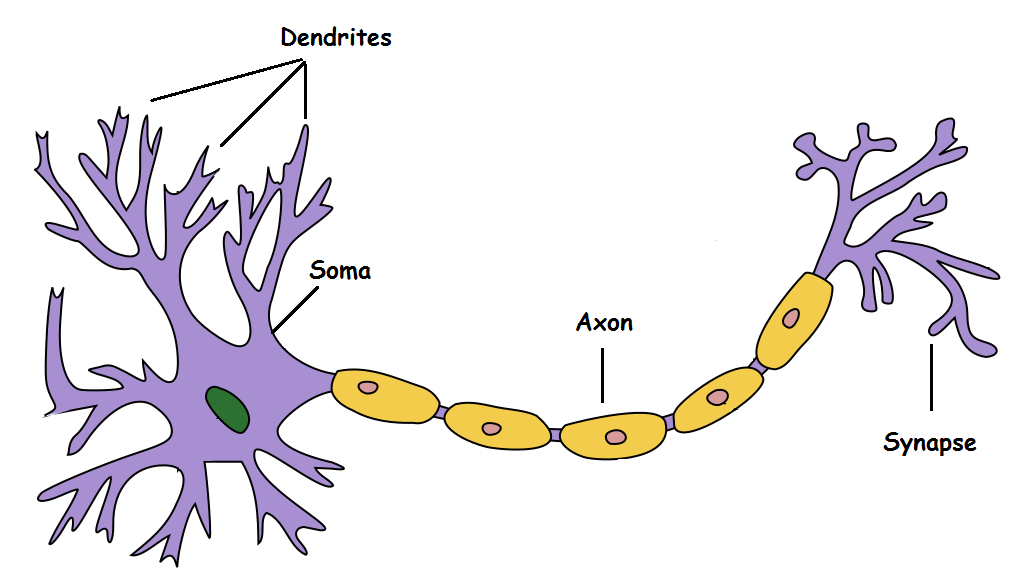
\includegraphics[width=\linewidth]{figs/neuron-bio.png}
	    \column{.3\textwidth}
			\includegraphics[width=\linewidth]{figs/sinapsis.jpg}
	    \column{.1\textwidth}
    \end{columns}
\end{frame}

\begin{frame}{Introduction}{Structure of neurons (III)}
	A neuron only fires if its input signal exceeds a threshold
	\begin{itemize}
	\item Good connections allowing a large signal
	\item Slight connections allowing a weak signal
	\item Synapses may be either excitatory or inhibitory
	\end{itemize}
	Synapses vary in strength
	\begin{itemize}
		\item Biological learning involves setting that strength
	\end{itemize}
\end{frame}

\section{Artificial neurons}

\subsection{Definition}

\begin{frame}{Artificial neurons}{Definition (I)}

    \input{figs/neuron.tex}

	\bigskip
    \begin{columns}
 	   \column{.70\textwidth}
		\begin{description}
		\item[$a_i$] Normalized input ($0 \le a_i \le 1$)
		\item[$w_{i}$] Weight of input $j$
		\item[$\theta$] Threshold
		\item[$g$] Activation function
		\end{description}

 	   \column{.30\textwidth}
	   \begin{block}{Neuron model (perceptron)}
	   \vspace{-0.5cm}
	   \begin{equation*}
	   y=g\left( \sum_{i=1}^n w_{i} a_i \right)
	   \end{equation*}
	   \end{block}
    \end{columns}
\end{frame}

\begin{frame}{Artificial neurons}{Definition (II)}
	\begin{itemize}
	\item Each neuron has a threshold value
	\item Each neuron has weighted inputs
	\item The input signals form a weighted sum
	\item If the activation level exceeds the threshold, the neuron activates
	\end{itemize}
\end{frame}

\begin{frame}{Artificial neurons}{Definition (III)}
	\begin{columns}
	\column{0.60\textwidth}
	The idealized activation function is a step function
	\begin{equation*}
	g(x) =
	  \begin{cases}
	      1  & \text{if } \sum_{i=1}^{N} w_i x_i > \theta\\
		  0  & \text{otherwise}\\
	  \end{cases}
	\end{equation*}
	The step function is rarely used in practice

	\column{0.30\textwidth}
    \begin{tikzpicture}[scale=0.4]
      \begin{axis}[ 
          xlabel=$x$,
          ylabel={$g(x)$},
		  xtick={2},
		  xticklabels={$\theta$}
      ] 
        %\addplot[mark=none] {2/(1+e^(-2*x))-1}; 
		\addplot[mark=none, red] coordinates {
			(-2,0)
			(2,0)
			(2,1)
			(6,1)
		};
        %\addplot {x^2 - x +4}; 
      \end{axis}
    \end{tikzpicture}
	\column{0.10\textwidth}
 	\end{columns}

\end{frame}

\subsection{Logical gates with a neuron}
\begin{frame}{Artificial neurons}{Logical gates with a neuron}
    \begin{columns}
 	   \column{.30\textwidth}
	   		\centering AND\\
            \input{figs/ann-and.tex}

			 \begin{tabular}{ccc}\hline
			 $a_1$ & $a_2$ & $y$ \\\hline
			 $0$ & $0$ & $0$ \\
			 $0$ & $1$ & $0$ \\
			 $1$ & $0$ & $0$ \\
			 $1$ & $1$ & $1$ \\
			 \end{tabular}
 	   \column{.30\textwidth}
	   		\centering OR\\
            \input{figs/ann-or.tex}

			 \begin{tabular}{ccc}\hline
			 $a_1$ & $a_2$ & $y$ \\\hline
			 $0$ & $0$ & $0$ \\
			 $0$ & $1$ & $1$ \\
			 $1$ & $0$ & $0$ \\
			 $1$ & $1$ & $1$ \\
			 \end{tabular}
 	   \column{.30\textwidth}
	   		\centering NOT\\\bigskip
            \input{figs/ann-not.tex}
			\vspace{1cm}
			 \begin{tabular}{cc}\hline
			 $a_1$ & $y$ \\\hline
			 $0$ & $1$ \\
			 $1$ & $0$ \\
			 \end{tabular}
    \end{columns}
	\bigskip
	\centering \href{https://github.com/dfbarrero/aiCourse/raw/master/ann/artificialNeuron.xlsx}{(A neuron in Excel)}
\end{frame}

\begin{frame}{Artificial neurons}{Definition of neuron (alternative version)}
    \input{figs/neuron-alternative.tex}

	\bigskip
    \begin{columns}
 	   \column{.70\textwidth}
		\begin{description}
		\item[$a_i$] Normalized input ($0 \le a_i \le 1$)
		\item[$w_{i}$] Weight of input $j$
		\item[$w_0$] Bias
		\item[$g$] Activation function
		\end{description}

 	   \column{.30\textwidth}
	   \begin{block}{Neuron model}
	   \vspace{-0.5cm}
	   \begin{equation*}
	   y=g\left( \sum_{i=0}^n w_{i} a_i \right)
	   \end{equation*}
	   \end{block}
    \end{columns}
\end{frame}

\begin{frame}{Artificial neurons}{Example of biased neuron}
	AND logical gate with a biased input

	\centering \input{figs/ann-and-biased.tex}

	\bigskip

	\centering \begin{tabular}{ccc|c}\hline
	$a_0$ & $a_1$ & $a_2$& Output\\\hline
	1    & 0     & 0     & 0\\
	1    & 0     & 1     & 0\\
	1    & 1     & 0     & 0\\
	1    & 1     & 1     & 1\\\hline
	\end{tabular}
\end{frame}

\subsection{Activation functions}
\begin{frame}{Artificial neurons}{Activation functions: Sigmoid function}
	\begin{itemize}
		\item Biological motivation
		\item S-shaped, continuous and everywhere differentiable
		\item Asymptotically approach saturation points
		\item Derivative fast computation
        \item Range $\in [0, 1]$
	\end{itemize}

	\medskip

	\begin{columns}[T]
 	   \column{.60\textwidth}

    		\begin{tikzpicture}[scale=0.5]
      			\begin{axis}[ 
          			xlabel=$x$,
          			ylabel={$g(x) = \frac{1}{1+e^{-x}}$}
      			] 
        		\addplot[mark=none, red] {1/(1+e^(-x))}; 
      			\end{axis}
    		\end{tikzpicture}
                      
                      
 	   \column{.40\textwidth}
		\vspace{-0.5cm}

		\begin{block}{Sigmoid function}
		\begin{equation*}
		g(x) = \frac{1}{1+e^{-x}}
		\end{equation*}
		\begin{equation*}
		g'(x) = g(x) (1-g(x))
		\end{equation*}
		\end{block}
    	\end{columns}
\end{frame}

\begin{frame}{Artificial neurons}{Activation functions: Tanh function}
    \begin{itemize}
	\item Asymptotically approach saturation points
        \item Range $\in [-1, 1]$
        \item Bigger derivative than sigmoid (faster training)
    \end{itemize}

    \begin{columns}[T]
 	\column{.50\textwidth}

     	    \begin{tikzpicture}[scale=0.5]
      		\begin{axis}[ 
          		xlabel=$x$,
          		ylabel={$g(x) = \tanh(x)$}
      		] 
        	\addplot[mark=none,red] {2/(1+e^(-2*x))-1}; 
        	%\addplot {x^2 - x +4}; 
      		\end{axis}
    		\end{tikzpicture}
                 
 	\column{.50\textwidth}
	    \begin{block}{Tanh function}
		\vspace{-0.5cm}

	        \begin{equation*}
	        g(x) = \tanh(x) = \frac{2}{1+e^{-2x}}-1
	        \end{equation*}
	        \begin{equation*}
           	g'(x) = 1 - g(x)^2
	        \end{equation*}
	    \end{block}
    \end{columns}
\end{frame}

\begin{frame}{Artificial neurons}{Activation functions: Softmax function}
	\begin{itemize}
		\item Generalization of the logistic function
		\item Usually used in the output layer in classification problems
		\item Asymptotically approach saturation points
	\end{itemize}

	\begin{columns}[T]
 	   \column{.60\textwidth}
	    \begin{block}{Softmax function}
	        \vspace{-0.25cm}

	        \begin{equation*}
	        g(\pmb z)_j = \frac{e^{z_j}}{\sum_{k=1}^{K}e^{z_k}} \text{ for } j=1, ...,K
	        \end{equation*}
	        with  \textbf{z} a K-dimensional vector
	    \end{block}
    \end{columns}
\end{frame}

\begin{frame}{Artificial neurons}{Other activation functions}
	\begin{columns}[T]
 	   \column{.30\textwidth}

		\centering Linear function
	    	\smallskip

    		\begin{tikzpicture}[scale=0.4]
      		\begin{axis}[ 
          		xlabel=$x$,
          		ylabel={$g(x) = x$}
      		] 
        		\addplot[mark=none,red] {x}; 
      		\end{axis}
    		\end{tikzpicture}

	   	\begin{itemize}
		   \item Used in regression
	   	\end{itemize}
 
 	   \column{.30\textwidth}
	   	\centering Rectified Linear (ReLU)
	    	\medskip

    		\begin{tikzpicture}[scale=0.4]
      		\begin{axis}[ 
          		xlabel=$x$,
          		ylabel={$g(x)$}
      		] 
		\addplot[mark=none, red] coordinates {
			(-6,0)
			(0,0)
			(6,6)
		};
      		\end{axis}
    		\end{tikzpicture}


	   	\begin{itemize}
		   \item Faster derivate
		   \item Popular in DL
	   	\end{itemize}

 	   \column{.30\textwidth}
	    \centering Leaky ReLU
	    \medskip

    		\begin{tikzpicture}[scale=0.4]
      		\begin{axis}[ 
          		xlabel=$x$,
          		ylabel={$g(x)$}
      		] 
		\addplot[mark=none, red] coordinates {
			(-6,-0.25)
			(0,0)
			(6,6)
		};
      		\end{axis}
    		\end{tikzpicture}

	   	\begin{itemize}
		   \item More informative derivate
		   \item Popular in DL
	   	\end{itemize}
    \end{columns}

    \bigskip
    The lack of non-linear activation function makes a network a simple linear regression
\end{frame}

\subsection{Learning limits}
\begin{frame}{Artificial neurons}{Learning limits (I)}
	\begin{center}
	\includegraphics[width=0.9\linewidth]{figs/linear2.png}
	\end{center}
	Problem: A single neuron only can solve linearly separable problems
	\note{Explicar sobre la pizarra funciones booleanas}
\end{frame}

\begin{frame}{Artificial neurons}{Learning limits (II)}
	XOR cannot be implemented with a neuron
	\begin{center}
	\includegraphics[width=0.7\linewidth]{figs/xor.jpg}
	\end{center}
	Solution: Neuronal networks
\end{frame}

\section{Artificial Neural Networks}
\subsection{Definition}

%\begin{frame}{Artificial Neural Networks}{Definition (I)}

%    \begin{columns}
% 	   \column{.80\textwidth}
%	\begin{itemize}
%	\item A very much simplified version of biological nerve systems
%	\item A set of nodes (neurons) 
%		\begin{itemize}
%		\item Each node has input and output
%		\item Each node performs a simple computation 
%		\end{itemize}
%	\item Weighted connections between nodes
%		\begin{itemize}
%		\item Connectivity gives the structure of the net
%		\item What can be computed by an ANN is primarily determined by the connections and their weights
%		\end{itemize}
%	\item It can \alert{recognize patterns}, \alert{learn} and \alert{generalize}
%	\end{itemize}

 %	   \column{.40\textwidth}
%	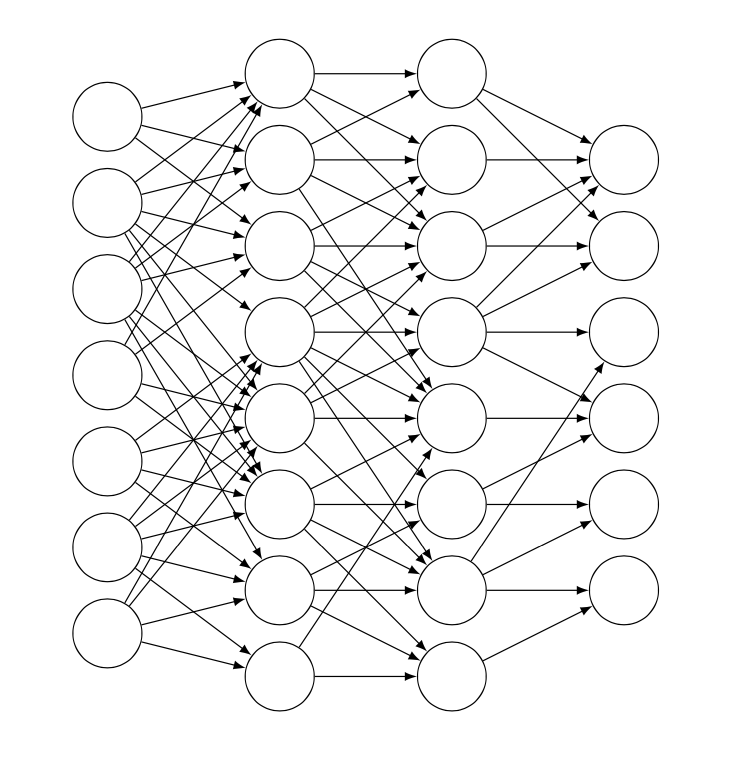
\includegraphics[width=\linewidth]{figs/network2.png}
%	\tiny{\href{https://tex.stackexchange.com/questions/540287/tikz-randomly-drop-connections-in-neural-network}{(Source)}}
 %   \end{columns}
%\end{frame}

\begin{frame}{Artificial Neural Networks}{Definition (II)}
	ANN properties
	\begin{itemize}
	\item Noise tolerance
	\item General function approximator
	\end{itemize}

	Machine Learning tasks
	\begin{itemize}
	\item Supervised learning (classification and regression)
	\item Unsupervised learning (known as \alert{self-organizing maps} in ANN terminology)
	\end{itemize}

	Many topologies
	\begin{itemize}
		\item Acyclic, recurrent (cyclic), modular, etc
		\item Feed Forward networks (MLPs)
	\end{itemize}

	\centering \textit{Human readability less important than performance}
\end{frame}

%\begin{frame}{Artificial Neural Networks}{What is a artificial neural network (III)}
\begin{frame}[plain]{}{}
\vspace{-0.2cm}
\begin{center}
    \begin{columns}
 	   \column{.2\textwidth}
	\href{http://www.asimovinstitute.org/neural-network-zoo/}{(More info)}
 	   \column{.8\textwidth}
	\includegraphics[width=0.7\linewidth]{figs/neuralnetworks.png}
	\end{columns}
\end{center}
\end{frame}

\subsection{Application examples}
\begin{frame}{Artificial Neural Networks}{Application examples (I)}
	\centering\includegraphics[width=0.9\linewidth]{figs/control.png}
\end{frame}

\begin{frame}{Artificial Neural Networks}{Application examples (II)}
	\centering\includegraphics[width=0.9\linewidth]{figs/robot.png}
\end{frame}

\begin{frame}{Artificial Neural Networks}{Application examples (III)}
    \begin{columns}
 	   \column{.5\textwidth}
	\centering\includegraphics[width=\linewidth]{figs/world.png}
 	   \column{.5\textwidth}
	\centering\includegraphics[width=\linewidth]{figs/worldann.png}
    \end{columns}
    \centering \scriptsize\href{https://en.wikibooks.org/wiki/Cyberbotics\%27\_Robot\_Curriculum/}{(Source)}
\end{frame}

\begin{frame}{Artificial Neural Networks}{Application examples (IV)}
	\centering\includegraphics[width=0.75\linewidth]{figs/autoencoder.png}\\\smallskip
	\centering\includegraphics[width=0.3\linewidth]{figs/autoencoder2.png}\\
	\scriptsize\href{http://i-systems.github.io/HSE545/machine\%20learning\%20all/KIMM/06\_KIMM\_Autoencoder.html}{(Source)}
\end{frame}

%\subsection{Topologies}
%\begin{frame}{Artificial Neural Networks}{Topologies (I)}
%    Acyclic Networks
%    \begin{itemize}
%        \item Without directed cycles 
%        \item Easy to analyze
%    \end{itemize}
%    Recurrent Networks
%    \begin{itemize}
%        \item With directed cycles
%        \item Much harder to analyze
%        \item Potentially unstable
%    \end{itemize}
%    Modular nets
%    \begin{itemize}
%        \item Consists of several modules
%        \item Each module is itself an ANN
%        \item Sparse connections between modules
%    \end{itemize}
%\end{frame}

%\begin{frame}{Artificial Neural Networks}{Topologies (II)}
%	Asymmetric fully connected networks
%		\begin{itemize}
%		\item Every node is connected to every other node
%		\item Connection may be excitatory (positive), inhibitory (negative), or irrelevant (0)
%		\item Most general
%		\end{itemize}
%		\vspace{-0.7cm}
%		\begin{center}
	%\includegraphics[width=0.5\linewidth]{figs/connected.png}
%	\end{center}
%		\vspace{-0.5cm}
%	Symmetric fully connected nets
%		\begin{itemize}
%		\item Weights are symmetric ($w_{ij}$ = $w_{ji}$)
%		\end{itemize}
%\end{frame}

%\subsection{Layered networks}
%\begin{frame}{Network architecture}{Layered networks (I)}
%		\begin{itemize}
%		\item Nodes are partitioned into subsets, called layers
%		\item No connections from nodes in layer $j$ to those in layer $k$ if $j > k$
%		\end{itemize}

%    \begin{columns}
% 	   \column{.50\textwidth}
%	\centering\includegraphics[width=\linewidth]{figs/layered.png}
% 	   \column{.50\textwidth}
%	   \begin{itemize}
%	   \item Inputs are applied to nodes in layer 0
%	   \item Nodes in input layer without computation
%	   \end{itemize}
%	   \end{columns}
%\end{frame}

%\begin{frame}{Network architecture}{Layered networks (II)}
%	\begin{center}
%	\alert{Perceptron}: ANN whose input is directly contected with its output
%	\includegraphics[width=0.5\linewidth]{figs/network.png}
%	\end{center}
%\end{frame}

\section{Feedforward networks}
\subsection{Definition}
\begin{frame}{Feedforward networks}{Definition (I)}
	Neurons are arranged in \alert{layers}
	\begin{description}
	\item[\textit{Input}] Which consists of any normalized data
	\item[\textit{Output}] Which are the net outcome
	\item[\textit{Hidden}] (Optional) No direct interaction
	\end{description}

	Also known as \textbf{multilayer perceptron} (MLP)

	\bigskip

    \begin{columns}
 	   \column{.2\textwidth}
 	   \column{.6\textwidth}
            %%%%%%%%%%%%%%%%%%%%%%%%%%%%%%%%%%%%%%%%%%%%%%%%%%%%%%%%%%%%%%%%%
% MUW Presentation
% LaTeX Template
% Version 1.0 (27/12/2016)
%
% License:
% CC BY-NC-SA 4.0 (http://creativecommons.org/licenses/by-nc-sa/3.0/)
%
% Created by:
% Nicolas Ballarini, CeMSIIS, Medical University of Vienna
% nicoballarini@gmail.com
% http://statistics.msi.meduniwien.ac.at/
%
% Customized for UAH by:
% David F. Barrero, Departamento de Automática, UAH
%%%%%%%%%%%%%%%%%%%%%%%%%%%%%%%%%%%%%%%%%%%%%%%%%%%%%%%%%%%%%%%%%

\documentclass[10pt,compress]{beamer} % Change 10pt to make fonts of a different size
\mode<presentation>

\usepackage[spanish]{babel}
\usepackage{fontspec}
\usepackage{tikz}
\usepackage{etoolbox}
\usepackage{xcolor}
\usepackage{xstring}
\usepackage{listings}
\usepackage{multicol}

% Custom packages
\usepackage{algpseudocode}
\usepackage{tikz}
\usepackage{pgfplots}
\def\layersep{2.5cm}
\usetikzlibrary{matrix,chains,positioning,decorations.pathreplacing,arrows}

\definecolor{dkgreen}{rgb}{0,0.6,0}
\definecolor{gray}{rgb}{0.5,0.5,0.5}
\definecolor{mauve}{rgb}{0.58,0,0.82}
 

\usetheme{UAH}
\usecolortheme{UAH}
\setbeamertemplate{navigation symbols}{} 
\setbeamertemplate{caption}[numbered]

%%%%%%%%%%%%%%%%%%%%%%%%%%%%%%%%%%%%%%%%%%%%%%%%%%%%%%%%%%%%%%%%%
%% Presentation Info
\title[Aritificial Neural Networks]{Artificial Neural Networks}
\author{\asignatura\\\carrera}
\institute{}
\date{Departamento de Automática}
%%%%%%%%%%%%%%%%%%%%%%%%%%%%%%%%%%%%%%%%%%%%%%%%%%%%%%%%%%%%%%%%%


%%%%%%%%%%%%%%%%%%%%%%%%%%%%%%%%%%%%%%%%%%%%%%%%%%%%%%%%%%%%%%%%%
%% Descomentar para habilitar barra de navegación superior
\setNavigation
%%%%%%%%%%%%%%%%%%%%%%%%%%%%%%%%%%%%%%%%%%%%%%%%%%%%%%%%%%%%%%%%%

%%%%%%%%%%%%%%%%%%%%%%%%%%%%%%%%%%%%%%%%%%%%%%%%%%%%%%%%%%%%%%%%%
%% Configuración de logotipos en portada
%% Opacidad de los logotipos
\newcommand{\opacidad}{1}
%% Descomentar para habilitar logotipo en pié de página de portada
\renewcommand{\logoUno}{Images/isg.png}
%% Descomentar para habilitar logotipo en pié de página de portada
%\renewcommand{\logoDos}{Images/CCLogo.png}
%% Descomentar para habilitar logotipo en pié de página de portada
%\renewcommand{\logoTres}{Images/ALogo.png}
%% Descomentar para habilitar logotipo en pié de página de portada
%\renewcommand{\logoCuatro}{Images/ELogo.png}
%%%%%%%%%%%%%%%%%%%%%%%%%%%%%%%%%%%%%%%%%%%%%%%%%%%%%%%%%%%%%%%%%

%%%%%%%%%%%%%%%%%%%%%%%%%%%%%%%%%%%%%%%%%%%%%%%%%%%%%%%%%%%%%%%%%
%% FOOTLINE
%% Comment/Uncomment the following blocks to modify the footline
%% content in the body slides. 


%% Option A: Title and institute
\footlineA
%% Option B: Author and institute
%\footlineB
%% Option C: Title, Author and institute
%\footlineC
%%%%%%%%%%%%%%%%%%%%%%%%%%%%%%%%%%%%%%%%%%%%%%%%%%%%%%%%%%%%%%%%%

\begin{document}

%%%%%%%%%%%%%%%%%%%%%%%%%%%%%%%%%%%%%%%%%%%%%%%%%%%%%%%%%%%%%%%%%
% Use this block for a blue title slide with modified footline
{\titlepageBlue
    \begin{frame}
        \titlepage
    \end{frame}
}

\institute{\asignatura}

\begin{frame}[plain]{}
   \begin{block}{Objectives}
      \begin{enumerate}
         \item Describe biological neurons and networks
         \item Basics of artifical neurons and networks
         \item Understand the role of trainning in ANNs
         \item Strengths and weaknesses of ANNs
      \end{enumerate} 
   \end{block}

   \begin{block}{Bibliography}
	\begin{itemize}
        \item A. Tettamanzi, M. Tomassini. \textit{Soft Computing. Integrating Evolutionary, Neural, and Fuzzy Systems}. Springer-Verlag. 2001
	    \item McCulloch, W. and Pitts, W. (1943). \textit{A logical calculus of the ideas immanent in nervous activity}. Bulletin of Mathematical Biophysics, 7:115 - 133. 
	    \item Rosenblatt, Frank.  (1958). \textit{The Perceptron: A Probabilistic Model for Information Storage and Organization in the Brain}. Psychological Review, 65:386-408
	\end{itemize}
   \end{block}
\end{frame}

{
\disableNavigation{white}
\begin{frame}[shrink]{Table of Contents}
 \frametitle{Table of Contents}

    \begin{multicols}{2}
    \tableofcontents
    \end{multicols}
  % You might wish to add the option [pausesections]
\end{frame}
}

\section{Introduction}

%\subsection{Machine Learning tasks}
%\begin{frame}{Introduction}{Machine Learning (I)}
%	Machine Learning studies how to build data-driven models
%	\begin{itemize}
%	\item \textbf{Supervised learning} The dataset contains output examples
%	\begin{flushleft}
%		\begin{itemize}
%		\item \textbf{Classification} The output is a category
%		\item \textbf{Regression} The output is a number
%		\end{itemize}
%		\end{flushleft}
%	\item \textbf{Unsupervised learning} (or \textit{clustering}) The dataset does not contain output examples
%	\item \textbf{Reinforcement learning} Maximize reward
%	\end{itemize}
%	ML is data-driven
%\end{frame}

%\begin{frame}[plain]{Introduction}{Machine Learning (II)}
%	\note{Comparar data-driven con programacion clasica}
%	\begin{center}
%	\vspace{-0.3cm}
%		\includegraphics[width=0.44\linewidth]{figs/lifecycle.png}
%	\end{center}
%\end{frame}


\subsection{History}
\begin{frame}{Introduction}{History}
    \begin{columns}
 	   \column{.80\textwidth}

	\begin{itemize}
	\item[1888] \textit{Ramón y Cajal}. Discovery of biological neurons
	\item[1943] \textit{McCulloch \& Pitts}. First neural network designers
	\item[1949] \textit{Hebb}. First learning rule
	\item[1958] \textit{Rosenblatt}. Perceptron
	\item[1969] \textit{Minsky \& Papert}.  Perceptron limitation - Death of ANN
	\note{Single layer perceonptrons cannot represent (learn) simple functions such as XOR
	Multi-layer of non-linear units may have greater power but there is no learning rule for such nets
	Scaling problem: connection weights may grow infinitely}
	\item[1986] \textit{Rumelhart et al}. Re-emergence of ANN: Backpropagation
	\note{Backpropagation learning for multi-layer feed forward nets (with non-linear, differentiable node functions)}
	\item[201x] Convolutional Neural Networks (CNNs) - Deep learning
	\item[2014] \textit{Goodfellow et al.} Generative Adversarial Networks (GANs)
	\end{itemize}

 	   \column{.20\textwidth}
		\includegraphics[width=\linewidth]{figs/neuron-ryc.jpg}
	   \end{columns}
\end{frame}

\subsection{Structure of neurons}
\begin{frame}{Introduction}{Structure of neurons (I)}
    \vspace{-0.3cm}
    \begin{columns}
 	   \column{.50\textwidth}
		\begin{tabular}{r|r}\hline
		\sc{Animal} & \sc{Neurons} \\\hline
		Sponge & 0 \\
		Roundworm & 302 \\
		Jellyfish & 800 \\
		Ant & 250,000 \\
		Cockroach & 1,000,000 \\
		Frog & 16,000,000 \\
		Mouse & 71,000,000 \\
		Cat & 760,000,000 \\
		Macaque & 6,376,000,000 \\
		Human & 86,000,000,000 \\
		Elephant & 267,000,000,000 \\\hline
		\end{tabular}

 	   \column{.50\textwidth}
	   \begin{block}{Human brain}
		Neuron switching time: ~ 0.001 s\\
  		Synapsis: ~10-100 thousand\\
   		Scene recognition time: ~0.1 s
	\end{block}

    \begin{center}
	        \includegraphics[width=0.9\linewidth]{figs/power.jpg}\\
	        \tiny{\href{http://www.sjef.nu/a-basic-introduction-to-singularity-skepticism/}{(Source)}}
	\end{center}
    \end{columns}
\end{frame}

\begin{frame}{Introduction}{Structure of neurons (II)}
	%\centering\includegraphics[width=0.7\linewidth]{figs/neuronabio.png}\\
	A neuron has a cell body ...
		\begin{itemize}
			\item ... a branching \textit{input} structure (dendrite) and 
			\item ... a branching \textit{output} structure (axon)
		\end{itemize}
	Axons connect to dendrites via \alert{synapses}

	\bigskip

	\begin{columns}[c]
	    \column{.1\textwidth}
	    \column{.50\textwidth}
			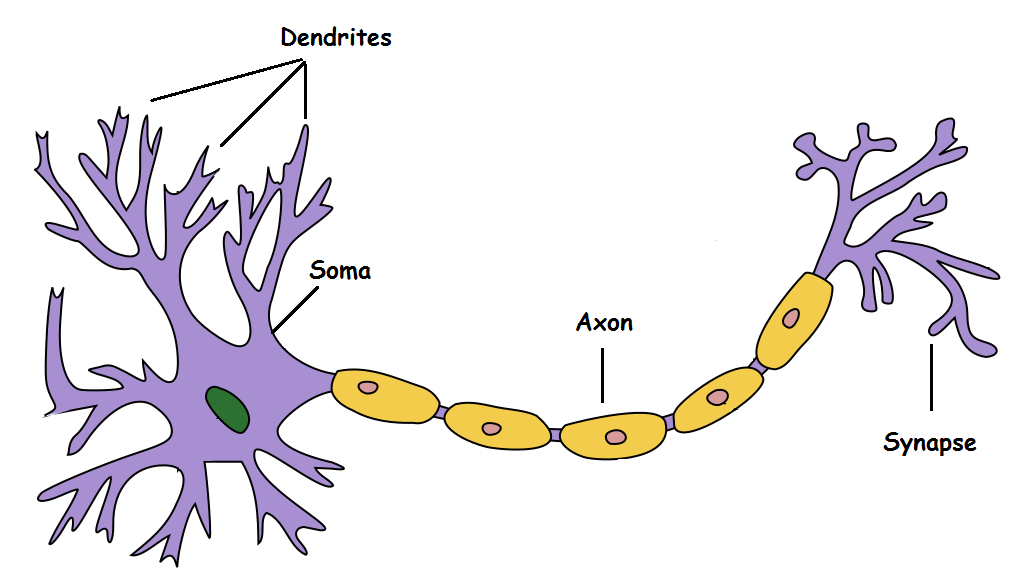
\includegraphics[width=\linewidth]{figs/neuron-bio.png}
	    \column{.3\textwidth}
			\includegraphics[width=\linewidth]{figs/sinapsis.jpg}
	    \column{.1\textwidth}
    \end{columns}
\end{frame}

\begin{frame}{Introduction}{Structure of neurons (III)}
	A neuron only fires if its input signal exceeds a threshold
	\begin{itemize}
	\item Good connections allowing a large signal
	\item Slight connections allowing a weak signal
	\item Synapses may be either excitatory or inhibitory
	\end{itemize}
	Synapses vary in strength
	\begin{itemize}
		\item Biological learning involves setting that strength
	\end{itemize}
\end{frame}

\section{Artificial neurons}

\subsection{Definition}

\begin{frame}{Artificial neurons}{Definition (I)}

    \input{figs/neuron.tex}

	\bigskip
    \begin{columns}
 	   \column{.70\textwidth}
		\begin{description}
		\item[$a_i$] Normalized input ($0 \le a_i \le 1$)
		\item[$w_{i}$] Weight of input $j$
		\item[$\theta$] Threshold
		\item[$g$] Activation function
		\end{description}

 	   \column{.30\textwidth}
	   \begin{block}{Neuron model (perceptron)}
	   \vspace{-0.5cm}
	   \begin{equation*}
	   y=g\left( \sum_{i=1}^n w_{i} a_i \right)
	   \end{equation*}
	   \end{block}
    \end{columns}
\end{frame}

\begin{frame}{Artificial neurons}{Definition (II)}
	\begin{itemize}
	\item Each neuron has a threshold value
	\item Each neuron has weighted inputs
	\item The input signals form a weighted sum
	\item If the activation level exceeds the threshold, the neuron activates
	\end{itemize}
\end{frame}

\begin{frame}{Artificial neurons}{Definition (III)}
	\begin{columns}
	\column{0.60\textwidth}
	The idealized activation function is a step function
	\begin{equation*}
	g(x) =
	  \begin{cases}
	      1  & \text{if } \sum_{i=1}^{N} w_i x_i > \theta\\
		  0  & \text{otherwise}\\
	  \end{cases}
	\end{equation*}
	The step function is rarely used in practice

	\column{0.30\textwidth}
    \begin{tikzpicture}[scale=0.4]
      \begin{axis}[ 
          xlabel=$x$,
          ylabel={$g(x)$},
		  xtick={2},
		  xticklabels={$\theta$}
      ] 
        %\addplot[mark=none] {2/(1+e^(-2*x))-1}; 
		\addplot[mark=none, red] coordinates {
			(-2,0)
			(2,0)
			(2,1)
			(6,1)
		};
        %\addplot {x^2 - x +4}; 
      \end{axis}
    \end{tikzpicture}
	\column{0.10\textwidth}
 	\end{columns}

\end{frame}

\subsection{Logical gates with a neuron}
\begin{frame}{Artificial neurons}{Logical gates with a neuron}
    \begin{columns}
 	   \column{.30\textwidth}
	   		\centering AND\\
            \input{figs/ann-and.tex}

			 \begin{tabular}{ccc}\hline
			 $a_1$ & $a_2$ & $y$ \\\hline
			 $0$ & $0$ & $0$ \\
			 $0$ & $1$ & $0$ \\
			 $1$ & $0$ & $0$ \\
			 $1$ & $1$ & $1$ \\
			 \end{tabular}
 	   \column{.30\textwidth}
	   		\centering OR\\
            \input{figs/ann-or.tex}

			 \begin{tabular}{ccc}\hline
			 $a_1$ & $a_2$ & $y$ \\\hline
			 $0$ & $0$ & $0$ \\
			 $0$ & $1$ & $1$ \\
			 $1$ & $0$ & $0$ \\
			 $1$ & $1$ & $1$ \\
			 \end{tabular}
 	   \column{.30\textwidth}
	   		\centering NOT\\\bigskip
            \input{figs/ann-not.tex}
			\vspace{1cm}
			 \begin{tabular}{cc}\hline
			 $a_1$ & $y$ \\\hline
			 $0$ & $1$ \\
			 $1$ & $0$ \\
			 \end{tabular}
    \end{columns}
	\bigskip
	\centering \href{https://github.com/dfbarrero/aiCourse/raw/master/ann/artificialNeuron.xlsx}{(A neuron in Excel)}
\end{frame}

\begin{frame}{Artificial neurons}{Definition of neuron (alternative version)}
    \input{figs/neuron-alternative.tex}

	\bigskip
    \begin{columns}
 	   \column{.70\textwidth}
		\begin{description}
		\item[$a_i$] Normalized input ($0 \le a_i \le 1$)
		\item[$w_{i}$] Weight of input $j$
		\item[$w_0$] Bias
		\item[$g$] Activation function
		\end{description}

 	   \column{.30\textwidth}
	   \begin{block}{Neuron model}
	   \vspace{-0.5cm}
	   \begin{equation*}
	   y=g\left( \sum_{i=0}^n w_{i} a_i \right)
	   \end{equation*}
	   \end{block}
    \end{columns}
\end{frame}

\begin{frame}{Artificial neurons}{Example of biased neuron}
	AND logical gate with a biased input

	\centering \input{figs/ann-and-biased.tex}

	\bigskip

	\centering \begin{tabular}{ccc|c}\hline
	$a_0$ & $a_1$ & $a_2$& Output\\\hline
	1    & 0     & 0     & 0\\
	1    & 0     & 1     & 0\\
	1    & 1     & 0     & 0\\
	1    & 1     & 1     & 1\\\hline
	\end{tabular}
\end{frame}

\subsection{Activation functions}
\begin{frame}{Artificial neurons}{Activation functions: Sigmoid function}
	\begin{itemize}
		\item Biological motivation
		\item S-shaped, continuous and everywhere differentiable
		\item Asymptotically approach saturation points
		\item Derivative fast computation
        \item Range $\in [0, 1]$
	\end{itemize}

	\medskip

	\begin{columns}[T]
 	   \column{.60\textwidth}

    		\begin{tikzpicture}[scale=0.5]
      			\begin{axis}[ 
          			xlabel=$x$,
          			ylabel={$g(x) = \frac{1}{1+e^{-x}}$}
      			] 
        		\addplot[mark=none, red] {1/(1+e^(-x))}; 
      			\end{axis}
    		\end{tikzpicture}
                      
                      
 	   \column{.40\textwidth}
		\vspace{-0.5cm}

		\begin{block}{Sigmoid function}
		\begin{equation*}
		g(x) = \frac{1}{1+e^{-x}}
		\end{equation*}
		\begin{equation*}
		g'(x) = g(x) (1-g(x))
		\end{equation*}
		\end{block}
    	\end{columns}
\end{frame}

\begin{frame}{Artificial neurons}{Activation functions: Tanh function}
    \begin{itemize}
	\item Asymptotically approach saturation points
        \item Range $\in [-1, 1]$
        \item Bigger derivative than sigmoid (faster training)
    \end{itemize}

    \begin{columns}[T]
 	\column{.50\textwidth}

     	    \begin{tikzpicture}[scale=0.5]
      		\begin{axis}[ 
          		xlabel=$x$,
          		ylabel={$g(x) = \tanh(x)$}
      		] 
        	\addplot[mark=none,red] {2/(1+e^(-2*x))-1}; 
        	%\addplot {x^2 - x +4}; 
      		\end{axis}
    		\end{tikzpicture}
                 
 	\column{.50\textwidth}
	    \begin{block}{Tanh function}
		\vspace{-0.5cm}

	        \begin{equation*}
	        g(x) = \tanh(x) = \frac{2}{1+e^{-2x}}-1
	        \end{equation*}
	        \begin{equation*}
           	g'(x) = 1 - g(x)^2
	        \end{equation*}
	    \end{block}
    \end{columns}
\end{frame}

\begin{frame}{Artificial neurons}{Activation functions: Softmax function}
	\begin{itemize}
		\item Generalization of the logistic function
		\item Usually used in the output layer in classification problems
		\item Asymptotically approach saturation points
	\end{itemize}

	\begin{columns}[T]
 	   \column{.60\textwidth}
	    \begin{block}{Softmax function}
	        \vspace{-0.25cm}

	        \begin{equation*}
	        g(\pmb z)_j = \frac{e^{z_j}}{\sum_{k=1}^{K}e^{z_k}} \text{ for } j=1, ...,K
	        \end{equation*}
	        with  \textbf{z} a K-dimensional vector
	    \end{block}
    \end{columns}
\end{frame}

\begin{frame}{Artificial neurons}{Other activation functions}
	\begin{columns}[T]
 	   \column{.30\textwidth}

		\centering Linear function
	    	\smallskip

    		\begin{tikzpicture}[scale=0.4]
      		\begin{axis}[ 
          		xlabel=$x$,
          		ylabel={$g(x) = x$}
      		] 
        		\addplot[mark=none,red] {x}; 
      		\end{axis}
    		\end{tikzpicture}

	   	\begin{itemize}
		   \item Used in regression
           \item Last layer in regression
	   	\end{itemize}
 
 	   \column{.30\textwidth}
	   	\centering Rectified Linear (ReLU)
	    	\medskip

    		\begin{tikzpicture}[scale=0.4]
      		\begin{axis}[ 
          		xlabel=$x$,
          		ylabel={$g(x)$}
      		] 
		\addplot[mark=none, red] coordinates {
			(-6,0)
			(0,0)
			(6,6)
		};
      		\end{axis}
    		\end{tikzpicture}


	   	\begin{itemize}
		   \item Faster derivate
		   \item Popular in DL
	   	\end{itemize}

 	   \column{.30\textwidth}
	    \centering Leaky ReLU
	    \medskip

    		\begin{tikzpicture}[scale=0.4]
      		\begin{axis}[ 
          		xlabel=$x$,
          		ylabel={$g(x)$}
      		] 
		\addplot[mark=none, red] coordinates {
			(-6,-0.25)
			(0,0)
			(6,6)
		};
      		\end{axis}
    		\end{tikzpicture}

	   	\begin{itemize}
		   \item More informative derivate
		   \item Popular in DL
	   	\end{itemize}
    \end{columns}

    \bigskip
    The lack of non-linear activation function makes a network a simple linear regression
\end{frame}

\subsection{Learning limits}
\begin{frame}{Artificial neurons}{Learning limits (I)}
	\begin{center}
	\includegraphics[width=0.9\linewidth]{figs/linear2.png}
	\end{center}
	Problem: A single neuron only can solve linearly separable problems
	\note{Explicar sobre la pizarra funciones booleanas}
\end{frame}

\begin{frame}{Artificial neurons}{Learning limits (II)}
	XOR cannot be implemented with a neuron
	\begin{center}
	\includegraphics[width=0.7\linewidth]{figs/xor.jpg}
	\end{center}
	Solution: Neuronal networks
\end{frame}

\section{Artificial Neural Networks}
\subsection{Definition}

\begin{frame}{Artificial Neural Networks}{Definition (I)}
    \begin{columns}
	   \column{.80\textwidth}
	\begin{itemize}
	\item A very much simplified version of biological nerve systems
	\item A set of nodes (neurons) 
		\begin{itemize}
		\item Each node has input and output
		\item Each node performs a simple computation 
		\end{itemize}
	\item Weighted connections between nodes
		\begin{itemize}
		\item Connectivity gives the structure of the net
		\item What can be computed by an ANN is primarily determined by the connections and their weights
		\end{itemize}
	\item It can \alert{recognize patterns}, \alert{learn} and \alert{generalize}
	\end{itemize}

 	   \column{.40\textwidth}
	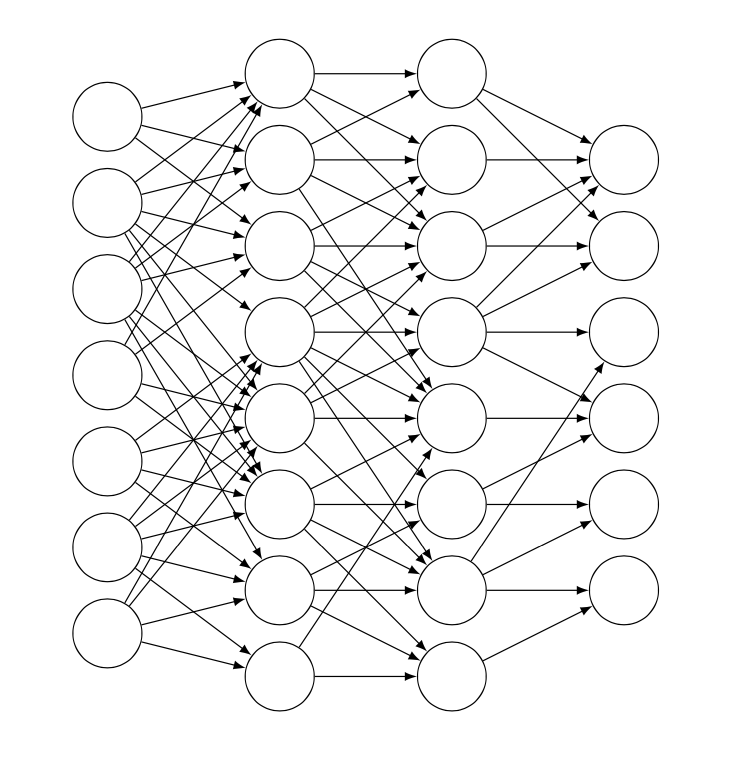
\includegraphics[width=\linewidth]{figs/network2.png}
	\tiny{\href{https://tex.stackexchange.com/questions/540287/tikz-randomly-drop-connections-in-neural-network}{(Source)}}
    \end{columns}
\end{frame}

\begin{frame}{Artificial Neural Networks}{Definition (II)}
	ANN properties
	\begin{itemize}
	\item Noise tolerance
	\item General function approximator
	\end{itemize}

	Machine Learning tasks
	\begin{itemize}
	\item Supervised learning (classification and regression)
	\item Unsupervised learning (known as \alert{self-organizing maps} in ANN terminology)
	\end{itemize}

	Many topologies
	\begin{itemize}
		\item Acyclic, recurrent (cyclic), modular, etc
		\item Feed Forward networks (MLPs)
	\end{itemize}

	\centering \textit{Human readability less important than performance}
\end{frame}

%\begin{frame}{Artificial Neural Networks}{What is a artificial neural network (III)}
\begin{frame}[plain]{}{}
\vspace{-0.2cm}
\begin{center}
    \begin{columns}
 	   \column{.2\textwidth}
	\href{http://www.asimovinstitute.org/neural-network-zoo/}{(More info)}
 	   \column{.8\textwidth}
	\includegraphics[width=0.7\linewidth]{figs/neuralnetworks.png}
	\end{columns}
\end{center}
\end{frame}

\subsection{Application examples}
\begin{frame}{Artificial Neural Networks}{Application examples (I)}
	\centering\includegraphics[width=0.9\linewidth]{figs/control.png}
\end{frame}

\begin{frame}{Artificial Neural Networks}{Application examples (II)}
	\centering\includegraphics[width=0.9\linewidth]{figs/robot.png}
\end{frame}

\begin{frame}{Artificial Neural Networks}{Application examples (III)}
    \begin{columns}
 	   \column{.5\textwidth}
	\centering\includegraphics[width=\linewidth]{figs/world.png}
 	   \column{.5\textwidth}
	\centering\includegraphics[width=\linewidth]{figs/worldann.png}
    \end{columns}
    \centering \scriptsize\href{https://en.wikibooks.org/wiki/Cyberbotics\%27\_Robot\_Curriculum/}{(Source)}
\end{frame}

\begin{frame}{Artificial Neural Networks}{Application examples (IV)}
	\centering\includegraphics[width=0.75\linewidth]{figs/autoencoder.png}\\\smallskip
	\centering\includegraphics[width=0.3\linewidth]{figs/autoencoder2.png}\\
	\scriptsize\href{http://i-systems.github.io/HSE545/machine\%20learning\%20all/KIMM/06\_KIMM\_Autoencoder.html}{(Source)}
\end{frame}

%\subsection{Topologies}
%\begin{frame}{Artificial Neural Networks}{Topologies (I)}
%    Acyclic Networks
%    \begin{itemize}
%        \item Without directed cycles 
%        \item Easy to analyze
%    \end{itemize}
%    Recurrent Networks
%    \begin{itemize}
%        \item With directed cycles
%        \item Much harder to analyze
%        \item Potentially unstable
%    \end{itemize}
%    Modular nets
%    \begin{itemize}
%        \item Consists of several modules
%        \item Each module is itself an ANN
%        \item Sparse connections between modules
%    \end{itemize}
%\end{frame}

%\begin{frame}{Artificial Neural Networks}{Topologies (II)}
%	Asymmetric fully connected networks
%		\begin{itemize}
%		\item Every node is connected to every other node
%		\item Connection may be excitatory (positive), inhibitory (negative), or irrelevant (0)
%		\item Most general
%		\end{itemize}
%		\vspace{-0.7cm}
%		\begin{center}
	%\includegraphics[width=0.5\linewidth]{figs/connected.png}
%	\end{center}
%		\vspace{-0.5cm}
%	Symmetric fully connected nets
%		\begin{itemize}
%		\item Weights are symmetric ($w_{ij}$ = $w_{ji}$)
%		\end{itemize}
%\end{frame}

%\subsection{Layered networks}
%\begin{frame}{Network architecture}{Layered networks (I)}
%		\begin{itemize}
%		\item Nodes are partitioned into subsets, called layers
%		\item No connections from nodes in layer $j$ to those in layer $k$ if $j > k$
%		\end{itemize}

%    \begin{columns}
% 	   \column{.50\textwidth}
%	\centering\includegraphics[width=\linewidth]{figs/layered.png}
% 	   \column{.50\textwidth}
%	   \begin{itemize}
%	   \item Inputs are applied to nodes in layer 0
%	   \item Nodes in input layer without computation
%	   \end{itemize}
%	   \end{columns}
%\end{frame}

%\begin{frame}{Network architecture}{Layered networks (II)}
%	\begin{center}
%	\alert{Perceptron}: ANN whose input is directly contected with its output
%	\includegraphics[width=0.5\linewidth]{figs/network.png}
%	\end{center}
%\end{frame}

\section{Feedforward networks}
\subsection{Definition}
\begin{frame}{Feedforward networks}{Definition (I)}
	Neurons are arranged in \alert{layers}
	\begin{description}
	\item[\textit{Input}] Which consists of any normalized data
	\item[\textit{Output}] Which are the net outcome
	\item[\textit{Hidden}] (Optional) No direct interaction
	\end{description}

	Also known as \textbf{multilayer perceptron} (MLP)

	\bigskip

    \begin{columns}
 	   \column{.2\textwidth}
 	   \column{.6\textwidth}
            %%%%%%%%%%%%%%%%%%%%%%%%%%%%%%%%%%%%%%%%%%%%%%%%%%%%%%%%%%%%%%%%%
% MUW Presentation
% LaTeX Template
% Version 1.0 (27/12/2016)
%
% License:
% CC BY-NC-SA 4.0 (http://creativecommons.org/licenses/by-nc-sa/3.0/)
%
% Created by:
% Nicolas Ballarini, CeMSIIS, Medical University of Vienna
% nicoballarini@gmail.com
% http://statistics.msi.meduniwien.ac.at/
%
% Customized for UAH by:
% David F. Barrero, Departamento de Automática, UAH
%%%%%%%%%%%%%%%%%%%%%%%%%%%%%%%%%%%%%%%%%%%%%%%%%%%%%%%%%%%%%%%%%

\documentclass[10pt,compress]{beamer} % Change 10pt to make fonts of a different size
\mode<presentation>

\usepackage[spanish]{babel}
\usepackage{fontspec}
\usepackage{tikz}
\usepackage{etoolbox}
\usepackage{xcolor}
\usepackage{xstring}
\usepackage{listings}
\usepackage{multicol}

% Custom packages
\usepackage{algpseudocode}
\usepackage{tikz}
\usepackage{pgfplots}
\def\layersep{2.5cm}
\usetikzlibrary{matrix,chains,positioning,decorations.pathreplacing,arrows}

\definecolor{dkgreen}{rgb}{0,0.6,0}
\definecolor{gray}{rgb}{0.5,0.5,0.5}
\definecolor{mauve}{rgb}{0.58,0,0.82}
 

\usetheme{UAH}
\usecolortheme{UAH}
\setbeamertemplate{navigation symbols}{} 
\setbeamertemplate{caption}[numbered]

%%%%%%%%%%%%%%%%%%%%%%%%%%%%%%%%%%%%%%%%%%%%%%%%%%%%%%%%%%%%%%%%%
%% Presentation Info
\title[Aritificial Neural Networks]{Artificial Neural Networks}
\author{\asignatura\\\carrera}
\institute{}
\date{Departamento de Automática}
%%%%%%%%%%%%%%%%%%%%%%%%%%%%%%%%%%%%%%%%%%%%%%%%%%%%%%%%%%%%%%%%%


%%%%%%%%%%%%%%%%%%%%%%%%%%%%%%%%%%%%%%%%%%%%%%%%%%%%%%%%%%%%%%%%%
%% Descomentar para habilitar barra de navegación superior
\setNavigation
%%%%%%%%%%%%%%%%%%%%%%%%%%%%%%%%%%%%%%%%%%%%%%%%%%%%%%%%%%%%%%%%%

%%%%%%%%%%%%%%%%%%%%%%%%%%%%%%%%%%%%%%%%%%%%%%%%%%%%%%%%%%%%%%%%%
%% Configuración de logotipos en portada
%% Opacidad de los logotipos
\newcommand{\opacidad}{1}
%% Descomentar para habilitar logotipo en pié de página de portada
\renewcommand{\logoUno}{Images/isg.png}
%% Descomentar para habilitar logotipo en pié de página de portada
%\renewcommand{\logoDos}{Images/CCLogo.png}
%% Descomentar para habilitar logotipo en pié de página de portada
%\renewcommand{\logoTres}{Images/ALogo.png}
%% Descomentar para habilitar logotipo en pié de página de portada
%\renewcommand{\logoCuatro}{Images/ELogo.png}
%%%%%%%%%%%%%%%%%%%%%%%%%%%%%%%%%%%%%%%%%%%%%%%%%%%%%%%%%%%%%%%%%

%%%%%%%%%%%%%%%%%%%%%%%%%%%%%%%%%%%%%%%%%%%%%%%%%%%%%%%%%%%%%%%%%
%% FOOTLINE
%% Comment/Uncomment the following blocks to modify the footline
%% content in the body slides. 


%% Option A: Title and institute
\footlineA
%% Option B: Author and institute
%\footlineB
%% Option C: Title, Author and institute
%\footlineC
%%%%%%%%%%%%%%%%%%%%%%%%%%%%%%%%%%%%%%%%%%%%%%%%%%%%%%%%%%%%%%%%%

\begin{document}

%%%%%%%%%%%%%%%%%%%%%%%%%%%%%%%%%%%%%%%%%%%%%%%%%%%%%%%%%%%%%%%%%
% Use this block for a blue title slide with modified footline
{\titlepageBlue
    \begin{frame}
        \titlepage
    \end{frame}
}

\institute{\asignatura}

\begin{frame}[plain]{}
   \begin{block}{Objectives}
      \begin{enumerate}
         \item Describe biological neurons and networks
         \item Basics of artifical neurons and networks
         \item Understand the role of trainning in ANNs
         \item Strengths and weaknesses of ANNs
      \end{enumerate} 
   \end{block}

   \begin{block}{Bibliography}
	\begin{itemize}
        \item A. Tettamanzi, M. Tomassini. \textit{Soft Computing. Integrating Evolutionary, Neural, and Fuzzy Systems}. Springer-Verlag. 2001
	    \item McCulloch, W. and Pitts, W. (1943). \textit{A logical calculus of the ideas immanent in nervous activity}. Bulletin of Mathematical Biophysics, 7:115 - 133. 
	    \item Rosenblatt, Frank.  (1958). \textit{The Perceptron: A Probabilistic Model for Information Storage and Organization in the Brain}. Psychological Review, 65:386-408
	\end{itemize}
   \end{block}
\end{frame}

{
\disableNavigation{white}
\begin{frame}[shrink]{Table of Contents}
 \frametitle{Table of Contents}

    \begin{multicols}{2}
    \tableofcontents
    \end{multicols}
  % You might wish to add the option [pausesections]
\end{frame}
}

\section{Introduction}

%\subsection{Machine Learning tasks}
%\begin{frame}{Introduction}{Machine Learning (I)}
%	Machine Learning studies how to build data-driven models
%	\begin{itemize}
%	\item \textbf{Supervised learning} The dataset contains output examples
%	\begin{flushleft}
%		\begin{itemize}
%		\item \textbf{Classification} The output is a category
%		\item \textbf{Regression} The output is a number
%		\end{itemize}
%		\end{flushleft}
%	\item \textbf{Unsupervised learning} (or \textit{clustering}) The dataset does not contain output examples
%	\item \textbf{Reinforcement learning} Maximize reward
%	\end{itemize}
%	ML is data-driven
%\end{frame}

%\begin{frame}[plain]{Introduction}{Machine Learning (II)}
%	\note{Comparar data-driven con programacion clasica}
%	\begin{center}
%	\vspace{-0.3cm}
%		\includegraphics[width=0.44\linewidth]{figs/lifecycle.png}
%	\end{center}
%\end{frame}


\subsection{History}
\begin{frame}{Introduction}{History}
    \begin{columns}
 	   \column{.80\textwidth}

	\begin{itemize}
	\item[1888] \textit{Ramón y Cajal}. Discovery of biological neurons
	\item[1943] \textit{McCulloch \& Pitts}. First neural network designers
	\item[1949] \textit{Hebb}. First learning rule
	\item[1958] \textit{Rosenblatt}. Perceptron
	\item[1969] \textit{Minsky \& Papert}.  Perceptron limitation - Death of ANN
	\note{Single layer perceonptrons cannot represent (learn) simple functions such as XOR
	Multi-layer of non-linear units may have greater power but there is no learning rule for such nets
	Scaling problem: connection weights may grow infinitely}
	\item[1986] \textit{Rumelhart et al}. Re-emergence of ANN: Backpropagation
	\note{Backpropagation learning for multi-layer feed forward nets (with non-linear, differentiable node functions)}
	\item[201x] Convolutional Neural Networks (CNNs) - Deep learning
	\item[2014] \textit{Goodfellow et al.} Generative Adversarial Networks (GANs)
	\end{itemize}

 	   \column{.20\textwidth}
		\includegraphics[width=\linewidth]{figs/neuron-ryc.jpg}
	   \end{columns}
\end{frame}

\subsection{Structure of neurons}
\begin{frame}{Introduction}{Structure of neurons (I)}
    \vspace{-0.3cm}
    \begin{columns}
 	   \column{.50\textwidth}
		\begin{tabular}{r|r}\hline
		\sc{Animal} & \sc{Neurons} \\\hline
		Sponge & 0 \\
		Roundworm & 302 \\
		Jellyfish & 800 \\
		Ant & 250,000 \\
		Cockroach & 1,000,000 \\
		Frog & 16,000,000 \\
		Mouse & 71,000,000 \\
		Cat & 760,000,000 \\
		Macaque & 6,376,000,000 \\
		Human & 86,000,000,000 \\
		Elephant & 267,000,000,000 \\\hline
		\end{tabular}

 	   \column{.50\textwidth}
	   \begin{block}{Human brain}
		Neuron switching time: ~ 0.001 s\\
  		Synapsis: ~10-100 thousand\\
   		Scene recognition time: ~0.1 s
	\end{block}

    \begin{center}
	        \includegraphics[width=0.9\linewidth]{figs/power.jpg}\\
	        \tiny{\href{http://www.sjef.nu/a-basic-introduction-to-singularity-skepticism/}{(Source)}}
	\end{center}
    \end{columns}
\end{frame}

\begin{frame}{Introduction}{Structure of neurons (II)}
	%\centering\includegraphics[width=0.7\linewidth]{figs/neuronabio.png}\\
	A neuron has a cell body ...
		\begin{itemize}
			\item ... a branching \textit{input} structure (dendrite) and 
			\item ... a branching \textit{output} structure (axon)
		\end{itemize}
	Axons connect to dendrites via \alert{synapses}

	\bigskip

	\begin{columns}[c]
	    \column{.1\textwidth}
	    \column{.50\textwidth}
			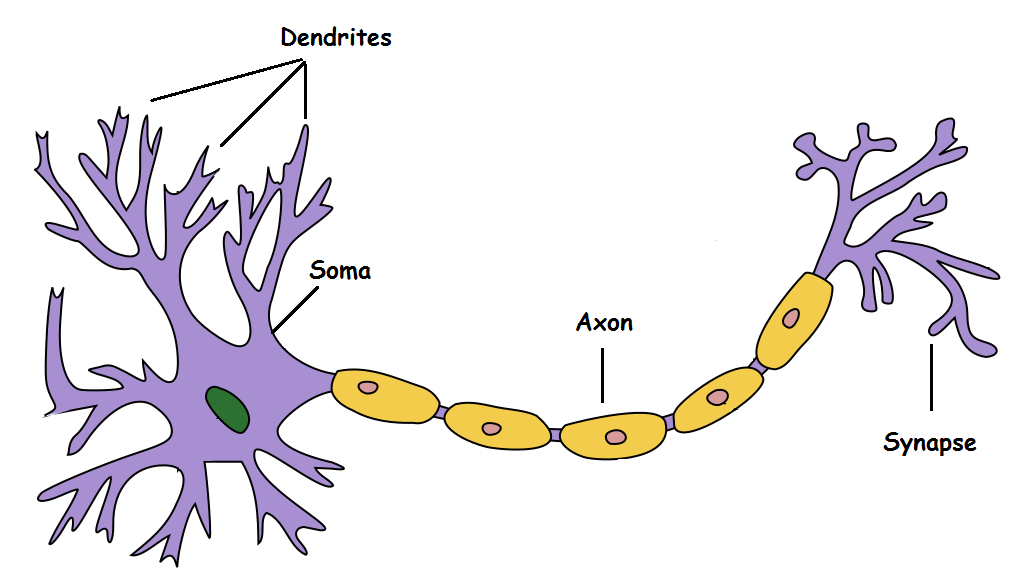
\includegraphics[width=\linewidth]{figs/neuron-bio.png}
	    \column{.3\textwidth}
			\includegraphics[width=\linewidth]{figs/sinapsis.jpg}
	    \column{.1\textwidth}
    \end{columns}
\end{frame}

\begin{frame}{Introduction}{Structure of neurons (III)}
	A neuron only fires if its input signal exceeds a threshold
	\begin{itemize}
	\item Good connections allowing a large signal
	\item Slight connections allowing a weak signal
	\item Synapses may be either excitatory or inhibitory
	\end{itemize}
	Synapses vary in strength
	\begin{itemize}
		\item Biological learning involves setting that strength
	\end{itemize}
\end{frame}

\section{Artificial neurons}

\subsection{Definition}

\begin{frame}{Artificial neurons}{Definition (I)}

    \input{figs/neuron.tex}

	\bigskip
    \begin{columns}
 	   \column{.70\textwidth}
		\begin{description}
		\item[$a_i$] Normalized input ($0 \le a_i \le 1$)
		\item[$w_{i}$] Weight of input $j$
		\item[$\theta$] Threshold
		\item[$g$] Activation function
		\end{description}

 	   \column{.30\textwidth}
	   \begin{block}{Neuron model (perceptron)}
	   \vspace{-0.5cm}
	   \begin{equation*}
	   y=g\left( \sum_{i=1}^n w_{i} a_i \right)
	   \end{equation*}
	   \end{block}
    \end{columns}
\end{frame}

\begin{frame}{Artificial neurons}{Definition (II)}
	\begin{itemize}
	\item Each neuron has a threshold value
	\item Each neuron has weighted inputs
	\item The input signals form a weighted sum
	\item If the activation level exceeds the threshold, the neuron activates
	\end{itemize}
\end{frame}

\begin{frame}{Artificial neurons}{Definition (III)}
	\begin{columns}
	\column{0.60\textwidth}
	The idealized activation function is a step function
	\begin{equation*}
	g(x) =
	  \begin{cases}
	      1  & \text{if } \sum_{i=1}^{N} w_i x_i > \theta\\
		  0  & \text{otherwise}\\
	  \end{cases}
	\end{equation*}
	The step function is rarely used in practice

	\column{0.30\textwidth}
    \begin{tikzpicture}[scale=0.4]
      \begin{axis}[ 
          xlabel=$x$,
          ylabel={$g(x)$},
		  xtick={2},
		  xticklabels={$\theta$}
      ] 
        %\addplot[mark=none] {2/(1+e^(-2*x))-1}; 
		\addplot[mark=none, red] coordinates {
			(-2,0)
			(2,0)
			(2,1)
			(6,1)
		};
        %\addplot {x^2 - x +4}; 
      \end{axis}
    \end{tikzpicture}
	\column{0.10\textwidth}
 	\end{columns}

\end{frame}

\subsection{Logical gates with a neuron}
\begin{frame}{Artificial neurons}{Logical gates with a neuron}
    \begin{columns}
 	   \column{.30\textwidth}
	   		\centering AND\\
            \input{figs/ann-and.tex}

			 \begin{tabular}{ccc}\hline
			 $a_1$ & $a_2$ & $y$ \\\hline
			 $0$ & $0$ & $0$ \\
			 $0$ & $1$ & $0$ \\
			 $1$ & $0$ & $0$ \\
			 $1$ & $1$ & $1$ \\
			 \end{tabular}
 	   \column{.30\textwidth}
	   		\centering OR\\
            \input{figs/ann-or.tex}

			 \begin{tabular}{ccc}\hline
			 $a_1$ & $a_2$ & $y$ \\\hline
			 $0$ & $0$ & $0$ \\
			 $0$ & $1$ & $1$ \\
			 $1$ & $0$ & $0$ \\
			 $1$ & $1$ & $1$ \\
			 \end{tabular}
 	   \column{.30\textwidth}
	   		\centering NOT\\\bigskip
            \input{figs/ann-not.tex}
			\vspace{1cm}
			 \begin{tabular}{cc}\hline
			 $a_1$ & $y$ \\\hline
			 $0$ & $1$ \\
			 $1$ & $0$ \\
			 \end{tabular}
    \end{columns}
	\bigskip
	\centering \href{https://github.com/dfbarrero/aiCourse/raw/master/ann/artificialNeuron.xlsx}{(A neuron in Excel)}
\end{frame}

\begin{frame}{Artificial neurons}{Definition of neuron (alternative version)}
    \input{figs/neuron-alternative.tex}

	\bigskip
    \begin{columns}
 	   \column{.70\textwidth}
		\begin{description}
		\item[$a_i$] Normalized input ($0 \le a_i \le 1$)
		\item[$w_{i}$] Weight of input $j$
		\item[$w_0$] Bias
		\item[$g$] Activation function
		\end{description}

 	   \column{.30\textwidth}
	   \begin{block}{Neuron model}
	   \vspace{-0.5cm}
	   \begin{equation*}
	   y=g\left( \sum_{i=0}^n w_{i} a_i \right)
	   \end{equation*}
	   \end{block}
    \end{columns}
\end{frame}

\begin{frame}{Artificial neurons}{Example of biased neuron}
	AND logical gate with a biased input

	\centering \input{figs/ann-and-biased.tex}

	\bigskip

	\centering \begin{tabular}{ccc|c}\hline
	$a_0$ & $a_1$ & $a_2$& Output\\\hline
	1    & 0     & 0     & 0\\
	1    & 0     & 1     & 0\\
	1    & 1     & 0     & 0\\
	1    & 1     & 1     & 1\\\hline
	\end{tabular}
\end{frame}

\subsection{Activation functions}
\begin{frame}{Artificial neurons}{Activation functions: Sigmoid function}
	\begin{itemize}
		\item Biological motivation
		\item S-shaped, continuous and everywhere differentiable
		\item Asymptotically approach saturation points
		\item Derivative fast computation
        \item Range $\in [0, 1]$
	\end{itemize}

	\medskip

	\begin{columns}[T]
 	   \column{.60\textwidth}

    		\begin{tikzpicture}[scale=0.5]
      			\begin{axis}[ 
          			xlabel=$x$,
          			ylabel={$g(x) = \frac{1}{1+e^{-x}}$}
      			] 
        		\addplot[mark=none, red] {1/(1+e^(-x))}; 
      			\end{axis}
    		\end{tikzpicture}
                      
                      
 	   \column{.40\textwidth}
		\vspace{-0.5cm}

		\begin{block}{Sigmoid function}
		\begin{equation*}
		g(x) = \frac{1}{1+e^{-x}}
		\end{equation*}
		\begin{equation*}
		g'(x) = g(x) (1-g(x))
		\end{equation*}
		\end{block}
    	\end{columns}
\end{frame}

\begin{frame}{Artificial neurons}{Activation functions: Tanh function}
    \begin{itemize}
	\item Asymptotically approach saturation points
        \item Range $\in [-1, 1]$
        \item Bigger derivative than sigmoid (faster training)
    \end{itemize}

    \begin{columns}[T]
 	\column{.50\textwidth}

     	    \begin{tikzpicture}[scale=0.5]
      		\begin{axis}[ 
          		xlabel=$x$,
          		ylabel={$g(x) = \tanh(x)$}
      		] 
        	\addplot[mark=none,red] {2/(1+e^(-2*x))-1}; 
        	%\addplot {x^2 - x +4}; 
      		\end{axis}
    		\end{tikzpicture}
                 
 	\column{.50\textwidth}
	    \begin{block}{Tanh function}
		\vspace{-0.5cm}

	        \begin{equation*}
	        g(x) = \tanh(x) = \frac{2}{1+e^{-2x}}-1
	        \end{equation*}
	        \begin{equation*}
           	g'(x) = 1 - g(x)^2
	        \end{equation*}
	    \end{block}
    \end{columns}
\end{frame}

\begin{frame}{Artificial neurons}{Activation functions: Softmax function}
	\begin{itemize}
		\item Generalization of the logistic function
		\item Usually used in the output layer in classification problems
		\item Asymptotically approach saturation points
	\end{itemize}

	\begin{columns}[T]
 	   \column{.60\textwidth}
	    \begin{block}{Softmax function}
	        \vspace{-0.25cm}

	        \begin{equation*}
	        g(\pmb z)_j = \frac{e^{z_j}}{\sum_{k=1}^{K}e^{z_k}} \text{ for } j=1, ...,K
	        \end{equation*}
	        with  \textbf{z} a K-dimensional vector
	    \end{block}
    \end{columns}
\end{frame}

\begin{frame}{Artificial neurons}{Other activation functions}
	\begin{columns}[T]
 	   \column{.30\textwidth}

		\centering Linear function
	    	\smallskip

    		\begin{tikzpicture}[scale=0.4]
      		\begin{axis}[ 
          		xlabel=$x$,
          		ylabel={$g(x) = x$}
      		] 
        		\addplot[mark=none,red] {x}; 
      		\end{axis}
    		\end{tikzpicture}

	   	\begin{itemize}
		   \item Used in regression
           \item Last layer in regression
	   	\end{itemize}
 
 	   \column{.30\textwidth}
	   	\centering Rectified Linear (ReLU)
	    	\medskip

    		\begin{tikzpicture}[scale=0.4]
      		\begin{axis}[ 
          		xlabel=$x$,
          		ylabel={$g(x)$}
      		] 
		\addplot[mark=none, red] coordinates {
			(-6,0)
			(0,0)
			(6,6)
		};
      		\end{axis}
    		\end{tikzpicture}


	   	\begin{itemize}
		   \item Faster derivate
		   \item Popular in DL
	   	\end{itemize}

 	   \column{.30\textwidth}
	    \centering Leaky ReLU
	    \medskip

    		\begin{tikzpicture}[scale=0.4]
      		\begin{axis}[ 
          		xlabel=$x$,
          		ylabel={$g(x)$}
      		] 
		\addplot[mark=none, red] coordinates {
			(-6,-0.25)
			(0,0)
			(6,6)
		};
      		\end{axis}
    		\end{tikzpicture}

	   	\begin{itemize}
		   \item More informative derivate
		   \item Popular in DL
	   	\end{itemize}
    \end{columns}

    \bigskip
    The lack of non-linear activation function makes a network a simple linear regression
\end{frame}

\subsection{Learning limits}
\begin{frame}{Artificial neurons}{Learning limits (I)}
	\begin{center}
	\includegraphics[width=0.9\linewidth]{figs/linear2.png}
	\end{center}
	Problem: A single neuron only can solve linearly separable problems
	\note{Explicar sobre la pizarra funciones booleanas}
\end{frame}

\begin{frame}{Artificial neurons}{Learning limits (II)}
	XOR cannot be implemented with a neuron
	\begin{center}
	\includegraphics[width=0.7\linewidth]{figs/xor.jpg}
	\end{center}
	Solution: Neuronal networks
\end{frame}

\section{Artificial Neural Networks}
\subsection{Definition}

\begin{frame}{Artificial Neural Networks}{Definition (I)}
    \begin{columns}
	   \column{.80\textwidth}
	\begin{itemize}
	\item A very much simplified version of biological nerve systems
	\item A set of nodes (neurons) 
		\begin{itemize}
		\item Each node has input and output
		\item Each node performs a simple computation 
		\end{itemize}
	\item Weighted connections between nodes
		\begin{itemize}
		\item Connectivity gives the structure of the net
		\item What can be computed by an ANN is primarily determined by the connections and their weights
		\end{itemize}
	\item It can \alert{recognize patterns}, \alert{learn} and \alert{generalize}
	\end{itemize}

 	   \column{.40\textwidth}
	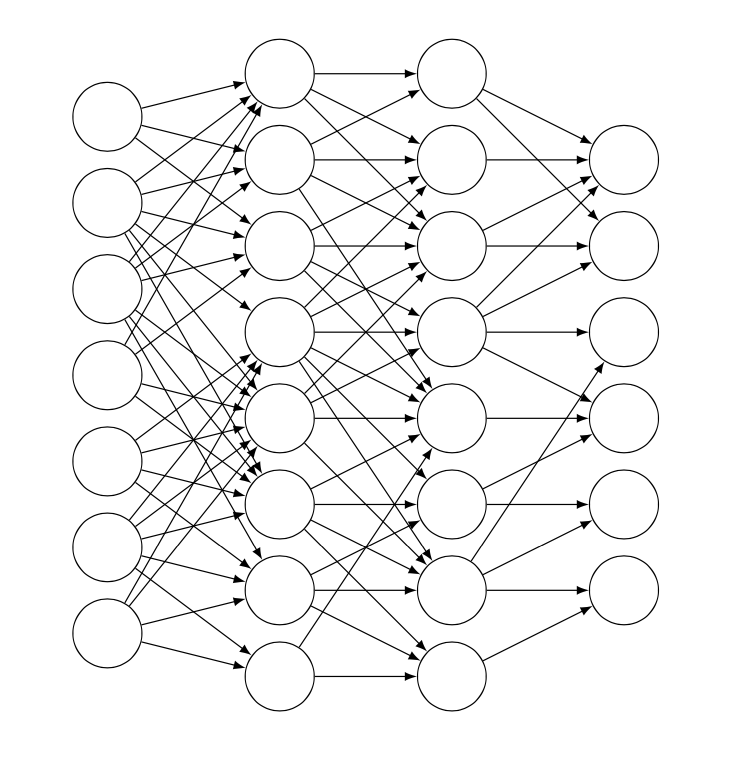
\includegraphics[width=\linewidth]{figs/network2.png}
	\tiny{\href{https://tex.stackexchange.com/questions/540287/tikz-randomly-drop-connections-in-neural-network}{(Source)}}
    \end{columns}
\end{frame}

\begin{frame}{Artificial Neural Networks}{Definition (II)}
	ANN properties
	\begin{itemize}
	\item Noise tolerance
	\item General function approximator
	\end{itemize}

	Machine Learning tasks
	\begin{itemize}
	\item Supervised learning (classification and regression)
	\item Unsupervised learning (known as \alert{self-organizing maps} in ANN terminology)
	\end{itemize}

	Many topologies
	\begin{itemize}
		\item Acyclic, recurrent (cyclic), modular, etc
		\item Feed Forward networks (MLPs)
	\end{itemize}

	\centering \textit{Human readability less important than performance}
\end{frame}

%\begin{frame}{Artificial Neural Networks}{What is a artificial neural network (III)}
\begin{frame}[plain]{}{}
\vspace{-0.2cm}
\begin{center}
    \begin{columns}
 	   \column{.2\textwidth}
	\href{http://www.asimovinstitute.org/neural-network-zoo/}{(More info)}
 	   \column{.8\textwidth}
	\includegraphics[width=0.7\linewidth]{figs/neuralnetworks.png}
	\end{columns}
\end{center}
\end{frame}

\subsection{Application examples}
\begin{frame}{Artificial Neural Networks}{Application examples (I)}
	\centering\includegraphics[width=0.9\linewidth]{figs/control.png}
\end{frame}

\begin{frame}{Artificial Neural Networks}{Application examples (II)}
	\centering\includegraphics[width=0.9\linewidth]{figs/robot.png}
\end{frame}

\begin{frame}{Artificial Neural Networks}{Application examples (III)}
    \begin{columns}
 	   \column{.5\textwidth}
	\centering\includegraphics[width=\linewidth]{figs/world.png}
 	   \column{.5\textwidth}
	\centering\includegraphics[width=\linewidth]{figs/worldann.png}
    \end{columns}
    \centering \scriptsize\href{https://en.wikibooks.org/wiki/Cyberbotics\%27\_Robot\_Curriculum/}{(Source)}
\end{frame}

\begin{frame}{Artificial Neural Networks}{Application examples (IV)}
	\centering\includegraphics[width=0.75\linewidth]{figs/autoencoder.png}\\\smallskip
	\centering\includegraphics[width=0.3\linewidth]{figs/autoencoder2.png}\\
	\scriptsize\href{http://i-systems.github.io/HSE545/machine\%20learning\%20all/KIMM/06\_KIMM\_Autoencoder.html}{(Source)}
\end{frame}

%\subsection{Topologies}
%\begin{frame}{Artificial Neural Networks}{Topologies (I)}
%    Acyclic Networks
%    \begin{itemize}
%        \item Without directed cycles 
%        \item Easy to analyze
%    \end{itemize}
%    Recurrent Networks
%    \begin{itemize}
%        \item With directed cycles
%        \item Much harder to analyze
%        \item Potentially unstable
%    \end{itemize}
%    Modular nets
%    \begin{itemize}
%        \item Consists of several modules
%        \item Each module is itself an ANN
%        \item Sparse connections between modules
%    \end{itemize}
%\end{frame}

%\begin{frame}{Artificial Neural Networks}{Topologies (II)}
%	Asymmetric fully connected networks
%		\begin{itemize}
%		\item Every node is connected to every other node
%		\item Connection may be excitatory (positive), inhibitory (negative), or irrelevant (0)
%		\item Most general
%		\end{itemize}
%		\vspace{-0.7cm}
%		\begin{center}
	%\includegraphics[width=0.5\linewidth]{figs/connected.png}
%	\end{center}
%		\vspace{-0.5cm}
%	Symmetric fully connected nets
%		\begin{itemize}
%		\item Weights are symmetric ($w_{ij}$ = $w_{ji}$)
%		\end{itemize}
%\end{frame}

%\subsection{Layered networks}
%\begin{frame}{Network architecture}{Layered networks (I)}
%		\begin{itemize}
%		\item Nodes are partitioned into subsets, called layers
%		\item No connections from nodes in layer $j$ to those in layer $k$ if $j > k$
%		\end{itemize}

%    \begin{columns}
% 	   \column{.50\textwidth}
%	\centering\includegraphics[width=\linewidth]{figs/layered.png}
% 	   \column{.50\textwidth}
%	   \begin{itemize}
%	   \item Inputs are applied to nodes in layer 0
%	   \item Nodes in input layer without computation
%	   \end{itemize}
%	   \end{columns}
%\end{frame}

%\begin{frame}{Network architecture}{Layered networks (II)}
%	\begin{center}
%	\alert{Perceptron}: ANN whose input is directly contected with its output
%	\includegraphics[width=0.5\linewidth]{figs/network.png}
%	\end{center}
%\end{frame}

\section{Feedforward networks}
\subsection{Definition}
\begin{frame}{Feedforward networks}{Definition (I)}
	Neurons are arranged in \alert{layers}
	\begin{description}
	\item[\textit{Input}] Which consists of any normalized data
	\item[\textit{Output}] Which are the net outcome
	\item[\textit{Hidden}] (Optional) No direct interaction
	\end{description}

	Also known as \textbf{multilayer perceptron} (MLP)

	\bigskip

    \begin{columns}
 	   \column{.2\textwidth}
 	   \column{.6\textwidth}
            %%%%%%%%%%%%%%%%%%%%%%%%%%%%%%%%%%%%%%%%%%%%%%%%%%%%%%%%%%%%%%%%%
% MUW Presentation
% LaTeX Template
% Version 1.0 (27/12/2016)
%
% License:
% CC BY-NC-SA 4.0 (http://creativecommons.org/licenses/by-nc-sa/3.0/)
%
% Created by:
% Nicolas Ballarini, CeMSIIS, Medical University of Vienna
% nicoballarini@gmail.com
% http://statistics.msi.meduniwien.ac.at/
%
% Customized for UAH by:
% David F. Barrero, Departamento de Automática, UAH
%%%%%%%%%%%%%%%%%%%%%%%%%%%%%%%%%%%%%%%%%%%%%%%%%%%%%%%%%%%%%%%%%

\documentclass[10pt,compress]{beamer} % Change 10pt to make fonts of a different size
\mode<presentation>

\usepackage[spanish]{babel}
\usepackage{fontspec}
\usepackage{tikz}
\usepackage{etoolbox}
\usepackage{xcolor}
\usepackage{xstring}
\usepackage{listings}
\usepackage{multicol}

% Custom packages
\usepackage{algpseudocode}
\usepackage{tikz}
\usepackage{pgfplots}
\def\layersep{2.5cm}
\usetikzlibrary{matrix,chains,positioning,decorations.pathreplacing,arrows}

\definecolor{dkgreen}{rgb}{0,0.6,0}
\definecolor{gray}{rgb}{0.5,0.5,0.5}
\definecolor{mauve}{rgb}{0.58,0,0.82}
 

\usetheme{UAH}
\usecolortheme{UAH}
\setbeamertemplate{navigation symbols}{} 
\setbeamertemplate{caption}[numbered]

%%%%%%%%%%%%%%%%%%%%%%%%%%%%%%%%%%%%%%%%%%%%%%%%%%%%%%%%%%%%%%%%%
%% Presentation Info
\title[Aritificial Neural Networks]{Artificial Neural Networks}
\author{\asignatura\\\carrera}
\institute{}
\date{Departamento de Automática}
%%%%%%%%%%%%%%%%%%%%%%%%%%%%%%%%%%%%%%%%%%%%%%%%%%%%%%%%%%%%%%%%%


%%%%%%%%%%%%%%%%%%%%%%%%%%%%%%%%%%%%%%%%%%%%%%%%%%%%%%%%%%%%%%%%%
%% Descomentar para habilitar barra de navegación superior
\setNavigation
%%%%%%%%%%%%%%%%%%%%%%%%%%%%%%%%%%%%%%%%%%%%%%%%%%%%%%%%%%%%%%%%%

%%%%%%%%%%%%%%%%%%%%%%%%%%%%%%%%%%%%%%%%%%%%%%%%%%%%%%%%%%%%%%%%%
%% Configuración de logotipos en portada
%% Opacidad de los logotipos
\newcommand{\opacidad}{1}
%% Descomentar para habilitar logotipo en pié de página de portada
\renewcommand{\logoUno}{Images/isg.png}
%% Descomentar para habilitar logotipo en pié de página de portada
%\renewcommand{\logoDos}{Images/CCLogo.png}
%% Descomentar para habilitar logotipo en pié de página de portada
%\renewcommand{\logoTres}{Images/ALogo.png}
%% Descomentar para habilitar logotipo en pié de página de portada
%\renewcommand{\logoCuatro}{Images/ELogo.png}
%%%%%%%%%%%%%%%%%%%%%%%%%%%%%%%%%%%%%%%%%%%%%%%%%%%%%%%%%%%%%%%%%

%%%%%%%%%%%%%%%%%%%%%%%%%%%%%%%%%%%%%%%%%%%%%%%%%%%%%%%%%%%%%%%%%
%% FOOTLINE
%% Comment/Uncomment the following blocks to modify the footline
%% content in the body slides. 


%% Option A: Title and institute
\footlineA
%% Option B: Author and institute
%\footlineB
%% Option C: Title, Author and institute
%\footlineC
%%%%%%%%%%%%%%%%%%%%%%%%%%%%%%%%%%%%%%%%%%%%%%%%%%%%%%%%%%%%%%%%%

\begin{document}

%%%%%%%%%%%%%%%%%%%%%%%%%%%%%%%%%%%%%%%%%%%%%%%%%%%%%%%%%%%%%%%%%
% Use this block for a blue title slide with modified footline
{\titlepageBlue
    \begin{frame}
        \titlepage
    \end{frame}
}

\institute{\asignatura}

\begin{frame}[plain]{}
   \begin{block}{Objectives}
      \begin{enumerate}
         \item Describe biological neurons and networks
         \item Basics of artifical neurons and networks
         \item Understand the role of trainning in ANNs
         \item Strengths and weaknesses of ANNs
      \end{enumerate} 
   \end{block}

   \begin{block}{Bibliography}
	\begin{itemize}
        \item A. Tettamanzi, M. Tomassini. \textit{Soft Computing. Integrating Evolutionary, Neural, and Fuzzy Systems}. Springer-Verlag. 2001
	    \item McCulloch, W. and Pitts, W. (1943). \textit{A logical calculus of the ideas immanent in nervous activity}. Bulletin of Mathematical Biophysics, 7:115 - 133. 
	    \item Rosenblatt, Frank.  (1958). \textit{The Perceptron: A Probabilistic Model for Information Storage and Organization in the Brain}. Psychological Review, 65:386-408
	\end{itemize}
   \end{block}
\end{frame}

{
\disableNavigation{white}
\begin{frame}[shrink]{Table of Contents}
 \frametitle{Table of Contents}

    \begin{multicols}{2}
    \tableofcontents
    \end{multicols}
  % You might wish to add the option [pausesections]
\end{frame}
}

\section{Introduction}

%\subsection{Machine Learning tasks}
%\begin{frame}{Introduction}{Machine Learning (I)}
%	Machine Learning studies how to build data-driven models
%	\begin{itemize}
%	\item \textbf{Supervised learning} The dataset contains output examples
%	\begin{flushleft}
%		\begin{itemize}
%		\item \textbf{Classification} The output is a category
%		\item \textbf{Regression} The output is a number
%		\end{itemize}
%		\end{flushleft}
%	\item \textbf{Unsupervised learning} (or \textit{clustering}) The dataset does not contain output examples
%	\item \textbf{Reinforcement learning} Maximize reward
%	\end{itemize}
%	ML is data-driven
%\end{frame}

%\begin{frame}[plain]{Introduction}{Machine Learning (II)}
%	\note{Comparar data-driven con programacion clasica}
%	\begin{center}
%	\vspace{-0.3cm}
%		\includegraphics[width=0.44\linewidth]{figs/lifecycle.png}
%	\end{center}
%\end{frame}


\subsection{History}
\begin{frame}{Introduction}{History}
    \begin{columns}
 	   \column{.80\textwidth}

	\begin{itemize}
	\item[1888] \textit{Ramón y Cajal}. Discovery of biological neurons
	\item[1943] \textit{McCulloch \& Pitts}. First neural network designers
	\item[1949] \textit{Hebb}. First learning rule
	\item[1958] \textit{Rosenblatt}. Perceptron
	\item[1969] \textit{Minsky \& Papert}.  Perceptron limitation - Death of ANN
	\note{Single layer perceonptrons cannot represent (learn) simple functions such as XOR
	Multi-layer of non-linear units may have greater power but there is no learning rule for such nets
	Scaling problem: connection weights may grow infinitely}
	\item[1986] \textit{Rumelhart et al}. Re-emergence of ANN: Backpropagation
	\note{Backpropagation learning for multi-layer feed forward nets (with non-linear, differentiable node functions)}
	\item[201x] Convolutional Neural Networks (CNNs) - Deep learning
	\item[2014] \textit{Goodfellow et al.} Generative Adversarial Networks (GANs)
	\end{itemize}

 	   \column{.20\textwidth}
		\includegraphics[width=\linewidth]{figs/neuron-ryc.jpg}
	   \end{columns}
\end{frame}

\subsection{Structure of neurons}
\begin{frame}{Introduction}{Structure of neurons (I)}
    \vspace{-0.3cm}
    \begin{columns}
 	   \column{.50\textwidth}
		\begin{tabular}{r|r}\hline
		\sc{Animal} & \sc{Neurons} \\\hline
		Sponge & 0 \\
		Roundworm & 302 \\
		Jellyfish & 800 \\
		Ant & 250,000 \\
		Cockroach & 1,000,000 \\
		Frog & 16,000,000 \\
		Mouse & 71,000,000 \\
		Cat & 760,000,000 \\
		Macaque & 6,376,000,000 \\
		Human & 86,000,000,000 \\
		Elephant & 267,000,000,000 \\\hline
		\end{tabular}

 	   \column{.50\textwidth}
	   \begin{block}{Human brain}
		Neuron switching time: ~ 0.001 s\\
  		Synapsis: ~10-100 thousand\\
   		Scene recognition time: ~0.1 s
	\end{block}

    \begin{center}
	        \includegraphics[width=0.9\linewidth]{figs/power.jpg}\\
	        \tiny{\href{http://www.sjef.nu/a-basic-introduction-to-singularity-skepticism/}{(Source)}}
	\end{center}
    \end{columns}
\end{frame}

\begin{frame}{Introduction}{Structure of neurons (II)}
	%\centering\includegraphics[width=0.7\linewidth]{figs/neuronabio.png}\\
	A neuron has a cell body ...
		\begin{itemize}
			\item ... a branching \textit{input} structure (dendrite) and 
			\item ... a branching \textit{output} structure (axon)
		\end{itemize}
	Axons connect to dendrites via \alert{synapses}

	\bigskip

	\begin{columns}[c]
	    \column{.1\textwidth}
	    \column{.50\textwidth}
			\includegraphics[width=\linewidth]{figs/neuron-bio.png}
	    \column{.3\textwidth}
			\includegraphics[width=\linewidth]{figs/sinapsis.jpg}
	    \column{.1\textwidth}
    \end{columns}
\end{frame}

\begin{frame}{Introduction}{Structure of neurons (III)}
	A neuron only fires if its input signal exceeds a threshold
	\begin{itemize}
	\item Good connections allowing a large signal
	\item Slight connections allowing a weak signal
	\item Synapses may be either excitatory or inhibitory
	\end{itemize}
	Synapses vary in strength
	\begin{itemize}
		\item Biological learning involves setting that strength
	\end{itemize}
\end{frame}

\section{Artificial neurons}

\subsection{Definition}

\begin{frame}{Artificial neurons}{Definition (I)}

    \input{figs/neuron.tex}

	\bigskip
    \begin{columns}
 	   \column{.70\textwidth}
		\begin{description}
		\item[$a_i$] Normalized input ($0 \le a_i \le 1$)
		\item[$w_{i}$] Weight of input $j$
		\item[$\theta$] Threshold
		\item[$g$] Activation function
		\end{description}

 	   \column{.30\textwidth}
	   \begin{block}{Neuron model (perceptron)}
	   \vspace{-0.5cm}
	   \begin{equation*}
	   y=g\left( \sum_{i=1}^n w_{i} a_i \right)
	   \end{equation*}
	   \end{block}
    \end{columns}
\end{frame}

\begin{frame}{Artificial neurons}{Definition (II)}
	\begin{itemize}
	\item Each neuron has a threshold value
	\item Each neuron has weighted inputs
	\item The input signals form a weighted sum
	\item If the activation level exceeds the threshold, the neuron activates
	\end{itemize}
\end{frame}

\begin{frame}{Artificial neurons}{Definition (III)}
	\begin{columns}
	\column{0.60\textwidth}
	The idealized activation function is a step function
	\begin{equation*}
	g(x) =
	  \begin{cases}
	      1  & \text{if } \sum_{i=1}^{N} w_i x_i > \theta\\
		  0  & \text{otherwise}\\
	  \end{cases}
	\end{equation*}
	The step function is rarely used in practice

	\column{0.30\textwidth}
    \begin{tikzpicture}[scale=0.4]
      \begin{axis}[ 
          xlabel=$x$,
          ylabel={$g(x)$},
		  xtick={2},
		  xticklabels={$\theta$}
      ] 
        %\addplot[mark=none] {2/(1+e^(-2*x))-1}; 
		\addplot[mark=none, red] coordinates {
			(-2,0)
			(2,0)
			(2,1)
			(6,1)
		};
        %\addplot {x^2 - x +4}; 
      \end{axis}
    \end{tikzpicture}
	\column{0.10\textwidth}
 	\end{columns}

\end{frame}

\subsection{Logical gates with a neuron}
\begin{frame}{Artificial neurons}{Logical gates with a neuron}
    \begin{columns}
 	   \column{.30\textwidth}
	   		\centering AND\\
            \input{figs/ann-and.tex}

			 \begin{tabular}{ccc}\hline
			 $a_1$ & $a_2$ & $y$ \\\hline
			 $0$ & $0$ & $0$ \\
			 $0$ & $1$ & $0$ \\
			 $1$ & $0$ & $0$ \\
			 $1$ & $1$ & $1$ \\
			 \end{tabular}
 	   \column{.30\textwidth}
	   		\centering OR\\
            \input{figs/ann-or.tex}

			 \begin{tabular}{ccc}\hline
			 $a_1$ & $a_2$ & $y$ \\\hline
			 $0$ & $0$ & $0$ \\
			 $0$ & $1$ & $1$ \\
			 $1$ & $0$ & $0$ \\
			 $1$ & $1$ & $1$ \\
			 \end{tabular}
 	   \column{.30\textwidth}
	   		\centering NOT\\\bigskip
            \input{figs/ann-not.tex}
			\vspace{1cm}
			 \begin{tabular}{cc}\hline
			 $a_1$ & $y$ \\\hline
			 $0$ & $1$ \\
			 $1$ & $0$ \\
			 \end{tabular}
    \end{columns}
	\bigskip
	\centering \href{https://github.com/dfbarrero/aiCourse/raw/master/ann/artificialNeuron.xlsx}{(A neuron in Excel)}
\end{frame}

\begin{frame}{Artificial neurons}{Definition of neuron (alternative version)}
    \input{figs/neuron-alternative.tex}

	\bigskip
    \begin{columns}
 	   \column{.70\textwidth}
		\begin{description}
		\item[$a_i$] Normalized input ($0 \le a_i \le 1$)
		\item[$w_{i}$] Weight of input $j$
		\item[$w_0$] Bias
		\item[$g$] Activation function
		\end{description}

 	   \column{.30\textwidth}
	   \begin{block}{Neuron model}
	   \vspace{-0.5cm}
	   \begin{equation*}
	   y=g\left( \sum_{i=0}^n w_{i} a_i \right)
	   \end{equation*}
	   \end{block}
    \end{columns}
\end{frame}

\begin{frame}{Artificial neurons}{Example of biased neuron}
	AND logical gate with a biased input

	\centering \input{figs/ann-and-biased.tex}

	\bigskip

	\centering \begin{tabular}{ccc|c}\hline
	$a_0$ & $a_1$ & $a_2$& Output\\\hline
	1    & 0     & 0     & 0\\
	1    & 0     & 1     & 0\\
	1    & 1     & 0     & 0\\
	1    & 1     & 1     & 1\\\hline
	\end{tabular}
\end{frame}

\subsection{Activation functions}
\begin{frame}{Artificial neurons}{Activation functions: Sigmoid function}
	\begin{itemize}
		\item Biological motivation
		\item S-shaped, continuous and everywhere differentiable
		\item Asymptotically approach saturation points
		\item Derivative fast computation
        \item Range $\in [0, 1]$
	\end{itemize}

	\medskip

	\begin{columns}[T]
 	   \column{.60\textwidth}

    		\begin{tikzpicture}[scale=0.5]
      			\begin{axis}[ 
          			xlabel=$x$,
          			ylabel={$g(x) = \frac{1}{1+e^{-x}}$}
      			] 
        		\addplot[mark=none, red] {1/(1+e^(-x))}; 
      			\end{axis}
    		\end{tikzpicture}
                      
                      
 	   \column{.40\textwidth}
		\vspace{-0.5cm}

		\begin{block}{Sigmoid function}
		\begin{equation*}
		g(x) = \frac{1}{1+e^{-x}}
		\end{equation*}
		\begin{equation*}
		g'(x) = g(x) (1-g(x))
		\end{equation*}
		\end{block}
    	\end{columns}
\end{frame}

\begin{frame}{Artificial neurons}{Activation functions: Tanh function}
    \begin{itemize}
	\item Asymptotically approach saturation points
        \item Range $\in [-1, 1]$
        \item Bigger derivative than sigmoid (faster training)
    \end{itemize}

    \begin{columns}[T]
 	\column{.50\textwidth}

     	    \begin{tikzpicture}[scale=0.5]
      		\begin{axis}[ 
          		xlabel=$x$,
          		ylabel={$g(x) = \tanh(x)$}
      		] 
        	\addplot[mark=none,red] {2/(1+e^(-2*x))-1}; 
        	%\addplot {x^2 - x +4}; 
      		\end{axis}
    		\end{tikzpicture}
                 
 	\column{.50\textwidth}
	    \begin{block}{Tanh function}
		\vspace{-0.5cm}

	        \begin{equation*}
	        g(x) = \tanh(x) = \frac{2}{1+e^{-2x}}-1
	        \end{equation*}
	        \begin{equation*}
           	g'(x) = 1 - g(x)^2
	        \end{equation*}
	    \end{block}
    \end{columns}
\end{frame}

\begin{frame}{Artificial neurons}{Activation functions: Softmax function}
	\begin{itemize}
		\item Generalization of the logistic function
		\item Usually used in the output layer in classification problems
		\item Asymptotically approach saturation points
	\end{itemize}

	\begin{columns}[T]
 	   \column{.60\textwidth}
	    \begin{block}{Softmax function}
	        \vspace{-0.25cm}

	        \begin{equation*}
	        g(\pmb z)_j = \frac{e^{z_j}}{\sum_{k=1}^{K}e^{z_k}} \text{ for } j=1, ...,K
	        \end{equation*}
	        with  \textbf{z} a K-dimensional vector
	    \end{block}
    \end{columns}
\end{frame}

\begin{frame}{Artificial neurons}{Other activation functions}
	\begin{columns}[T]
 	   \column{.30\textwidth}

		\centering Linear function
	    	\smallskip

    		\begin{tikzpicture}[scale=0.4]
      		\begin{axis}[ 
          		xlabel=$x$,
          		ylabel={$g(x) = x$}
      		] 
        		\addplot[mark=none,red] {x}; 
      		\end{axis}
    		\end{tikzpicture}

	   	\begin{itemize}
		   \item Used in regression
           \item Last layer in regression
	   	\end{itemize}
 
 	   \column{.30\textwidth}
	   	\centering Rectified Linear (ReLU)
	    	\medskip

    		\begin{tikzpicture}[scale=0.4]
      		\begin{axis}[ 
          		xlabel=$x$,
          		ylabel={$g(x)$}
      		] 
		\addplot[mark=none, red] coordinates {
			(-6,0)
			(0,0)
			(6,6)
		};
      		\end{axis}
    		\end{tikzpicture}


	   	\begin{itemize}
		   \item Faster derivate
		   \item Popular in DL
	   	\end{itemize}

 	   \column{.30\textwidth}
	    \centering Leaky ReLU
	    \medskip

    		\begin{tikzpicture}[scale=0.4]
      		\begin{axis}[ 
          		xlabel=$x$,
          		ylabel={$g(x)$}
      		] 
		\addplot[mark=none, red] coordinates {
			(-6,-0.25)
			(0,0)
			(6,6)
		};
      		\end{axis}
    		\end{tikzpicture}

	   	\begin{itemize}
		   \item More informative derivate
		   \item Popular in DL
	   	\end{itemize}
    \end{columns}

    \bigskip
    The lack of non-linear activation function makes a network a simple linear regression
\end{frame}

\subsection{Learning limits}
\begin{frame}{Artificial neurons}{Learning limits (I)}
	\begin{center}
	\includegraphics[width=0.9\linewidth]{figs/linear2.png}
	\end{center}
	Problem: A single neuron only can solve linearly separable problems
	\note{Explicar sobre la pizarra funciones booleanas}
\end{frame}

\begin{frame}{Artificial neurons}{Learning limits (II)}
	XOR cannot be implemented with a neuron
	\begin{center}
	\includegraphics[width=0.7\linewidth]{figs/xor.jpg}
	\end{center}
	Solution: Neuronal networks
\end{frame}

\section{Artificial Neural Networks}
\subsection{Definition}

\begin{frame}{Artificial Neural Networks}{Definition (I)}
    \begin{columns}
	   \column{.80\textwidth}
	\begin{itemize}
	\item A very much simplified version of biological nerve systems
	\item A set of nodes (neurons) 
		\begin{itemize}
		\item Each node has input and output
		\item Each node performs a simple computation 
		\end{itemize}
	\item Weighted connections between nodes
		\begin{itemize}
		\item Connectivity gives the structure of the net
		\item What can be computed by an ANN is primarily determined by the connections and their weights
		\end{itemize}
	\item It can \alert{recognize patterns}, \alert{learn} and \alert{generalize}
	\end{itemize}

 	   \column{.40\textwidth}
	\includegraphics[width=\linewidth]{figs/network2.png}
	\tiny{\href{https://tex.stackexchange.com/questions/540287/tikz-randomly-drop-connections-in-neural-network}{(Source)}}
    \end{columns}
\end{frame}

\begin{frame}{Artificial Neural Networks}{Definition (II)}
	ANN properties
	\begin{itemize}
	\item Noise tolerance
	\item General function approximator
	\end{itemize}

	Machine Learning tasks
	\begin{itemize}
	\item Supervised learning (classification and regression)
	\item Unsupervised learning (known as \alert{self-organizing maps} in ANN terminology)
	\end{itemize}

	Many topologies
	\begin{itemize}
		\item Acyclic, recurrent (cyclic), modular, etc
		\item Feed Forward networks (MLPs)
	\end{itemize}

	\centering \textit{Human readability less important than performance}
\end{frame}

%\begin{frame}{Artificial Neural Networks}{What is a artificial neural network (III)}
\begin{frame}[plain]{}{}
\vspace{-0.2cm}
\begin{center}
    \begin{columns}
 	   \column{.2\textwidth}
	\href{http://www.asimovinstitute.org/neural-network-zoo/}{(More info)}
 	   \column{.8\textwidth}
	\includegraphics[width=0.7\linewidth]{figs/neuralnetworks.png}
	\end{columns}
\end{center}
\end{frame}

\subsection{Application examples}
\begin{frame}{Artificial Neural Networks}{Application examples (I)}
	\centering\includegraphics[width=0.9\linewidth]{figs/control.png}
\end{frame}

\begin{frame}{Artificial Neural Networks}{Application examples (II)}
	\centering\includegraphics[width=0.9\linewidth]{figs/robot.png}
\end{frame}

\begin{frame}{Artificial Neural Networks}{Application examples (III)}
    \begin{columns}
 	   \column{.5\textwidth}
	\centering\includegraphics[width=\linewidth]{figs/world.png}
 	   \column{.5\textwidth}
	\centering\includegraphics[width=\linewidth]{figs/worldann.png}
    \end{columns}
    \centering \scriptsize\href{https://en.wikibooks.org/wiki/Cyberbotics\%27\_Robot\_Curriculum/}{(Source)}
\end{frame}

\begin{frame}{Artificial Neural Networks}{Application examples (IV)}
	\centering\includegraphics[width=0.75\linewidth]{figs/autoencoder.png}\\\smallskip
	\centering\includegraphics[width=0.3\linewidth]{figs/autoencoder2.png}\\
	\scriptsize\href{http://i-systems.github.io/HSE545/machine\%20learning\%20all/KIMM/06\_KIMM\_Autoencoder.html}{(Source)}
\end{frame}

%\subsection{Topologies}
%\begin{frame}{Artificial Neural Networks}{Topologies (I)}
%    Acyclic Networks
%    \begin{itemize}
%        \item Without directed cycles 
%        \item Easy to analyze
%    \end{itemize}
%    Recurrent Networks
%    \begin{itemize}
%        \item With directed cycles
%        \item Much harder to analyze
%        \item Potentially unstable
%    \end{itemize}
%    Modular nets
%    \begin{itemize}
%        \item Consists of several modules
%        \item Each module is itself an ANN
%        \item Sparse connections between modules
%    \end{itemize}
%\end{frame}

%\begin{frame}{Artificial Neural Networks}{Topologies (II)}
%	Asymmetric fully connected networks
%		\begin{itemize}
%		\item Every node is connected to every other node
%		\item Connection may be excitatory (positive), inhibitory (negative), or irrelevant (0)
%		\item Most general
%		\end{itemize}
%		\vspace{-0.7cm}
%		\begin{center}
	%\includegraphics[width=0.5\linewidth]{figs/connected.png}
%	\end{center}
%		\vspace{-0.5cm}
%	Symmetric fully connected nets
%		\begin{itemize}
%		\item Weights are symmetric ($w_{ij}$ = $w_{ji}$)
%		\end{itemize}
%\end{frame}

%\subsection{Layered networks}
%\begin{frame}{Network architecture}{Layered networks (I)}
%		\begin{itemize}
%		\item Nodes are partitioned into subsets, called layers
%		\item No connections from nodes in layer $j$ to those in layer $k$ if $j > k$
%		\end{itemize}

%    \begin{columns}
% 	   \column{.50\textwidth}
%	\centering\includegraphics[width=\linewidth]{figs/layered.png}
% 	   \column{.50\textwidth}
%	   \begin{itemize}
%	   \item Inputs are applied to nodes in layer 0
%	   \item Nodes in input layer without computation
%	   \end{itemize}
%	   \end{columns}
%\end{frame}

%\begin{frame}{Network architecture}{Layered networks (II)}
%	\begin{center}
%	\alert{Perceptron}: ANN whose input is directly contected with its output
%	\includegraphics[width=0.5\linewidth]{figs/network.png}
%	\end{center}
%\end{frame}

\section{Feedforward networks}
\subsection{Definition}
\begin{frame}{Feedforward networks}{Definition (I)}
	Neurons are arranged in \alert{layers}
	\begin{description}
	\item[\textit{Input}] Which consists of any normalized data
	\item[\textit{Output}] Which are the net outcome
	\item[\textit{Hidden}] (Optional) No direct interaction
	\end{description}

	Also known as \textbf{multilayer perceptron} (MLP)

	\bigskip

    \begin{columns}
 	   \column{.2\textwidth}
 	   \column{.6\textwidth}
            \input{figs/ann.tex}
 	   \column{.2\textwidth}
    \end{columns}
\end{frame}

\begin{frame}{Feedforward networks}{Definition (II)}
	The input layer
	\begin{itemize}
	\item Introduces input values into the network
	\item No activation function or other processing
	\end{itemize}
	The hidden layer(s)
	\begin{itemize}
	\item Perform classification of features
	\item Two hidden layers are sufficient to solve any problem
	\item Features imply more layers may be better
	\end{itemize}
	The output layer
	\begin{itemize}
	\item Functionally just like the hidden layers
	\item Outputs are passed on to the world outside the neural network
	\end{itemize}
\end{frame}

\subsection{Demo}
\begin{frame}{Feedforward Networks}{Demo}
    \begin{center}
	\href{http://playground.tensorflow.org/}{(Online demo)}
    \end{center}
\end{frame}

\subsection{Separability}
\begin{frame}{Feedforward Networks}{Separability}
    \begin{center}
	    \includegraphics[width=0.9\linewidth]{figs/sep.png}
    \end{center}

	\centering \href{https://github.com/dfbarrero/aiCourse/raw/master/ann/artificialNeuron.xlsx}{(A MLP in Excel)}
\end{frame}

\subsection{Bias in a MLP}
\begin{frame}{Feedforward Networks}{Bias in a MLP}
    \begin{center}
	    \includegraphics[width=0.6\paperheight]{figs/bias.png}\\
		\tiny \href{https://scikit-learn.org/stable/modules/neural\_networks\_supervised.html}{(Source)}
    \end{center}
\end{frame}


\section{Training algorithms}
\subsection{Problem statement}

\begin{frame}{Training algorithms}{Problem statement (I)}
    ANNs can perform different tasks
    \begin{itemize}
        \item Classification, regression, others
    \end{itemize}
    Classification (or supervised learning) uses a \textit{training set}

	\begin{columns}[c]
 	   \column{.10\textwidth}
 	   \column{.50\textwidth}
            \input{figs/ann-optimization.tex}

 	   \column{.40\textwidth}
            \begin{table}[]
            \centering
            \begin{tabular}{lll|l|l}\hline
              $A_1$ & $A_2$ & $A_3$ & O & Y \\
               \hline
              $1.1$ & $2.5$ & $4.5$ & $0.2$ & $-0.1$   \\
              $0.9$ & $2.4$ & $1.2$ & $0.5$ & $0.4$  \\
              $1.0$ & $2.0$ & $9.9$ & $0.4$ & $1.2$ \\\hline
            \end{tabular}
            \end{table}
 	   \column{.10\textwidth}
    \end{columns}
    Toss function: Measure of the error
        \begin{itemize}
        	\item Y and O are the desired and observed outputs
		\item Usually mean squared error (MSE): $f(w) = E = \frac{1}{2} (y-o)^2$
        \end{itemize}
\end{frame}

\subsection{Gradient descent algorithm}
\begin{frame}{Training algorithms}{Problem statement (II)}
		%\begin{equation*}
		%E = \frac{1}{2} Err^2 = \frac{1}{2} \left[y-g\left(\sum_{j=0}^n w_j x_j\right)\right]^2
		%\end{equation*}
		%where
		%\begin{flushleft}
		%\begin{itemize}
		%\item[$y$] Desired output
		%\item[$w_j$] Weight connection $j$
		%\item[$x_j$] Input $j$
		%\end{itemize}
		%\end{flushleft}

		Problem: Determine $\vec{w}$ that minimize $f(\vec{w})$
		\begin{itemize}
			\item Remember, $\vec{w}$ is our network
			\item This is a classical optimization problem
			\item Any optimization algorithm can be used
			\item ... in AI, optimization means search
		\end{itemize}
		We do know anatically $f(\vec{w})$ $\Rightarrow$ Optimization based on gradients
\end{frame}

\begin{frame}[fragile]{Training algorithms}{Gradient Descent (I)}
	Calculate the gradient of the loss function with respect weights
	\begin{itemize}
		\item Adjust weights along gradient direction
		\item Gradient provides the direction
		\item $\alpha$ is the \alert{learning rate} ($|\alpha|<1$)
	\end{itemize}

	\begin{columns}[c]
 	   \column{.50\textwidth}

		\begin{block}{Gradient descent}
		\begin{algorithmic}[1]
		\State $\vec{w} \gets random()$
		\While{Not converged}
			\ForAll {$w_i \in \vec{w} $}
			\State $w_i \gets w_i - \alpha \frac{\partial}{\partial w_i} f(\vec{w})$
			\EndFor
		\EndWhile
		\end{algorithmic}

		\end{block}

 	   \column{.10\textwidth}
 	   \column{.40\textwidth}

		\includegraphics[width=\linewidth]{figs/descent.png}\\

	\end{columns}
\end{frame}


%\begin{frame}{Training algorithms}{Gradient Descent (I)}
%	Calculate the gradient of the loss function with respect weights
%	\begin{itemize}
%		\item Adjust weights along gradient direction
%		\item Apply the chain rule
%	\end{itemize}
%	Given the error
%		\begin{equation*}
%		E = \frac{1}{2} Err^2
%		\end{equation*}
%	Take partial derivatives
%		\begin{equation*}
%		\begin{split}
%		\frac{\partial E}{\partial w_j} &= Err \frac{\partial Err}{\partial w_j}\\
%										&= Err \frac{\partial}{\partial w_j} g\left(y-\sum_{j=0}^n w_j x_j\right)\\
%										&= -Err \times g'(w) \times x_j
%		\end{split}
%		\end{equation*}
%\end{frame}



%\begin{frame}{Training algorithms}{Gradient Descent (II)}
%	\small{
%	\begin{columns}
%	\column{0.50\textwidth}
%		Weight update
%		\begin{equation*}
%		w_{j}^{k+1} = w_{j}^k + \alpha \times Err \times g'(w) \times x_j
%		\end{equation*}
%		with
%		\begin{flushleft}
%		\begin{itemize}
%		\item[$\alpha$] Learning rate ($|\alpha|<1$)
%		\item[$err$] Difference desired and current output
%		\item[$g'$] Derivate of activation function
%		\item[$x_j$] Input $j$
%		\end{itemize}
%		\end{flushleft}
%		Each iteration is named \alert{epoch}
%	\column{0.50\textwidth}
%		\begin{block}{Learning algorithm (single neuron)}
%		\begin{enumerate}
%		\item Apply input signal and compute outout
%		\item If output $==$ desired output, do nothing
%		\item If output $<$ desired output, increase weights
%		\item If output $>$ desired output, decrease weights
%		\end{enumerate}
%		\end{block}
%	\end{columns}
%	}
%\end{frame}

\begin{frame}{Training algorithms}{Gradient Descent (II)}
    \begin{columns}
    \column{0.50\textwidth}
	Each iteration is named \alert{epoch}
	\begin{center}
	\includegraphics[width=\linewidth]{figs/nn_learncurve.png}\\
	\scriptsize \href{http://sujitpal.blogspot.com.es/2014/07/handwritten-digit-recognition-with.html}{(Source)}
	\end{center}

    \column{0.50\textwidth}
	\vspace{-0.5cm}
	\begin{center}
        Learning rate\\
	\includegraphics[width=0.8\linewidth]{figs/nn_learning.png}\\
	\includegraphics[width=0.8\linewidth]{figs/nn_learning2.png}\\
	\scriptsize \href{http://www.turingfinance.com/misconceptions-about-neural-networks/}{(Source)}
	\end{center}
     \end{columns}
\end{frame}

\subsection{Stochastic Gradient Descent}
\begin{frame}{Training algorithms}{Stochastic Gradient Descent (I)}
	SDG approximates the gradient sampling the dataset
		\begin{description}
		\item[On-line] One sample
		\item[Mini-batch] Several samples
		\item[Batch] All the samples (Gradient Descent)
		\end{description}
	%Weights update rule: $w^{k+1} = w^k - \alpha \nabla g(in)$
	%	\begin{itemize}
	%		\item where $\alpha$ is the learning rate
	%	\end{itemize}
    	Computations are faster ...
	\begin{itemize}
		\item ... but gradient estimation looses accuracy
	\end{itemize}

	\centering
	\includegraphics[width=0.4\linewidth]{figs/sdg.png}\\
	\scriptsize \href{https://wikidocs.net/3413}{(Source)}
\end{frame}

\begin{frame}{Training algorithms}{Stochastic Gradient Descent (II)}
    Usually, a \alert{momentum} is introduced as
	\begin{equation*}
	w^{k+1} = w^k - \alpha z^{k+1}
        \end{equation*}
with
	\begin{equation*}
	z^{k+1} = \beta z^k + \nabla g(in)
        \end{equation*}
    where ...
    \begin{itemize}
	\item $\alpha$ is the learning rate
	\item $\beta$ is the momentum strength
        \item If $\beta = 0$ then gradient descent
    \end{itemize}

    \href{http://distill.pub/2017/momentum/}{(On-line demo)}

\end{frame}

\subsection{Other optimization algorithms}
\begin{frame}{Training algorithms}{Other optimization algorithms (I)}
	\begin{columns}
	\column{0.50\textwidth}
		Other second derivative-based optimization algorithms
		\begin{itemize}
			\item Newton's method
			\item Quasi-Newton's method
			\item Levenberg-Marquardt method
			\item Conjugate Gradient
		\end{itemize}

	\column{0.50\textwidth}
		\begin{center}
			\includegraphics[width=\linewidth]{figs/memory-speed.png}\\
			\scriptsize \href{https://www.neuraldesigner.com/blog/5_algorithms_to_train_a_neural_network}{(Source)}
		\end{center}
	\end{columns}
\end{frame}

\begin{frame}{Training algorithms}{Other optimization algorithms (II)}
	Learning reate / momentum  adaptative methods
	\begin{itemize}
		\item AdaGrad - Adaptative Gradient Algorithm
		\item RMSProp - Root Mean Square Propagation
		\item Adam - Adaptive Moment Estimation
	\end{itemize}
\end{frame}

\subsection{Backpropagation}

%\begin{frame}{Training algorithms}{Backpropagation algorithm (I)}
%Efficient learning algorithm for multilayer perceptrons. Three steps
%\begin{enumerate}
%\item \textbf{Feed-forward step}. Feed input, compute output and error
%\item \textbf{Feed-backward step}. Compute individual contribution to error
%\item \textbf{Adjust weights}. Modify weights to minimize error: Input, output and hidden layers
%\end{enumerate}
%\end{frame}

%\begin{frame}{Training algorithms}{Backpropagation algorithm (II)}
%    \begin{columns}
% 	   \column{.50\textwidth}
%	\centering\includegraphics[width=\linewidth]{figs/russell.png}
%
% 	   \column{.50\textwidth}
%	Output layer: Same as single neuron
%	\begin{equation*}
%	W_j \leftarrow W_j + \alpha \times Err \times g'(in) \times x_j
%	\end{equation*}
%	Define modified error as $\Delta_i = Err_i \times g'(in_i) $, then
%	\begin{equation*}
%	W_{j,i} \leftarrow W_{j,i} + \alpha \times a_j \times \Delta_i
%	\end{equation*}
%	\end{columns}
%\end{frame}

\begin{frame}{Training algorithms}{Backpropagation}
%Hidden layer: Propagate error
%\begin{equation*}
%W_{k,j} \leftarrow W_{k,j} + \alpha \times a_k \times \Delta_j
%\end{equation*}
%where
%\begin{equation*}
%\Delta_j = g'(in) \times \sum_j W_{j,i}\Delta_i
%\end{equation*}

        Backpropagation is an efficient algorithm to compute gradients
        \begin{itemize}
                \item It applyes the chain rule to propagate errors
		\item Implicit in optimization algorithms
        \end{itemize}

	\begin{block}{Backpropagation algorithm}
	\begin{enumerate}
	\item Compute output
	\item Compute error
	\item For each layer, repeat the following steps
	\begin{enumerate}
		\item Propagate errors backwards
		\item Update weights between two layers
	\end{enumerate}
	\end{enumerate}
	\end{block}
\end{frame}

%\subsection{Backpropagation algorithm formalization}
%\begin{frame}{Training algorithms}{Backpropagation algorithm formalization (I)}
%Network error: $E = \frac{1}{2} \sum_j (y_{i} - a_i)^2$, with
%\begin{flushleft}
%\begin{description}
%	\item{$E$} network error
%	\item{$y_{i}$} desired output at neuron $i$
%	\item{$a_{i}$} actual output at neuron $j$
%\end{description}
%\end{flushleft}
%Single neuron activation
%\begin{equation*}
%a_i=g\left(\sum_i w_{ij} a_j\right)
%\end{equation*}
%\begin{flushleft}
%\begin{description}
%	\item{$w_{ij}$} weight between neurons $i$ and $j$
%	\item{$o_{pi}$} activation from output $i$
%\end{description}
%\end{flushleft}
%and its output $o_{pj} = f_j(net_{pj})$
%\end{frame}

%\begin{frame}{Training algorithms}{Backpropagation algorithm formalization (II)}
%We try to minimize error in the output layer, so
%\begin{equation*}
%\begin{split}
%\frac{\partial E}{\partial W_{j,i}} & = \frac{\partial}{\partial W_{j,i}}\left[ \frac{1}{2} \sum_i (y_i-a_i)^2\right] = -(y_i-a_i) \frac{\partial a_i}{\partial W_{j,i}}\\
% & =  -(y_i-a_i) \frac{\partial g(in_i)}{\partial W_{j,i}} = -(y_i-a_i) g'(in) \frac{\partial in_i}{\partial W_{j,i}} \\
% & = -(y_i-a_i) g'(in) \frac{\partial }{\partial W_{j,i}} \left( \sum_j W_{j,i} a_j \right) \\
% & = -(y_i-a_i) g'(in) a_j = -a_j \Delta_i
%\end{split}
%\end{equation*}
%\end{frame}

%\begin{frame}[plain]{Training algorithms}{Backpropagation algorithm formalization (III)}
%\note{Las entradas ak influyen en las activaciones de aj, por lo que los errores se deben sumar. De ahi viene el sumatorio que aparece}
%Similarly, we minimize error in the hidden layer
%\small
%\begin{equation*}
%\begin{split}
%\frac{\partial E}{\partial W_{k,j}} & = -\sum_i(y_i-a_i) \frac{\partial a_i}{\partial W_{k,j}}\\
% & =  -\sum_i(y_i-a_i) \frac{\partial g(in_i)}{\partial W_{k,j}} = -\sum_i(y_i-a_i) g'(in) \frac{\partial in_i}{\partial W_{k,j}} \\
% & = -\sum_i \Delta_i \frac{\partial }{\partial W_{k,j}} \left( \sum_j W_{j,i} a_j \right) \\
% & = -\sum_i \Delta_i W_{j,i} \frac{\partial a_j}{\partial W_{k,j}} = -\sum_i \Delta_i W_{j,i}\frac{\partial g(in_i)}{\partial W_{k,j}}\\
% & = - \sum_i \Delta_i W_{j,i} g'(in) \frac{\partial in_j}{\partial W_{k,j}} = - \sum_i \Delta_i W_{j,i} g'(in) \frac{\partial}{\partial W_{k,j}}\left(\sum_k W_{k,j} a_k\right)\\
% & = - \sum_i \Delta_i W_{j,i} g'(in) a_k = -a_k \Delta_i
%\end{split}
%\end{equation*}
%\end{frame}

\subsection{Learning problems}
\begin{frame}{Training algorithms}{Learning problems}
    \begin{columns}
	   \column{.40\textwidth}
		Potential problems
		\begin{itemize}
		\item Local minima
		\item Flat plateau
		\item Oscillation
		\item Missing good minima
		\end{itemize}

	   \column{.60\textwidth}
	 \begin{center}
	\includegraphics[width=\linewidth]{figs/problems.png}
 	\end{center}
   \end{columns}
\end{frame}

\begin{frame}{Training algorithms}{Learning problems: Under and overfitting (I)}
    \begin{columns}
	   \column{.50\textwidth}
		\alert{Underfitting}: Does not learn
            \begin{itemize}
                \item Topology too simple
            \end{itemize}

		\alert{Overfitting}: Memorizes samples
            \begin{itemize}
                \item Topology too complex
                \item Perhaps, the most serious concern in ML
                \item The net fails when exposed to new data
            \end{itemize}

	   \column{.50\textwidth}
            \begin{center}
			\includegraphics[width=\linewidth]{figs/fitting.jpg}\\
			\scriptsize \href{https://www.youtube.com/watch?v=dBLZg-RqoLg}{(Source)}
            \end{center}
   \end{columns}
\end{frame}

\begin{frame}{Training algorithms}{Learning problems: Under and overfitting (II)}
       Solution: Evaluate generalization capabilities
            \begin{itemize}
                \item Split training and validation sets and measure errors
            \end{itemize}

            \begin{center}
			\includegraphics[width=0.6\linewidth]{figs/validation.png}\\
			\scriptsize \href{https://datascience.stackexchange.com/questions/61/why-is-overfitting-bad-in-machine-learning}{(Source)}
            \end{center}
\end{frame}

\begin{frame}{Acknowlegements}
	\begin{itemize}
		\item Jesus Aguilar Ruiz, Pablo de Olavide, Seville, Spain
		\item Daniel Rodr\'iguez, Universidad de Alcal\'a, Alcal\'a de Henares, Spain
	\end{itemize}
\end{frame}


\end{document}

 	   \column{.2\textwidth}
    \end{columns}
\end{frame}

\begin{frame}{Feedforward networks}{Definition (II)}
	The input layer
	\begin{itemize}
	\item Introduces input values into the network
	\item No activation function or other processing
	\end{itemize}
	The hidden layer(s)
	\begin{itemize}
	\item Perform classification of features
	\item Two hidden layers are sufficient to solve any problem
	\item Features imply more layers may be better
	\end{itemize}
	The output layer
	\begin{itemize}
	\item Functionally just like the hidden layers
	\item Outputs are passed on to the world outside the neural network
	\end{itemize}
\end{frame}

\subsection{Demo}
\begin{frame}{Feedforward Networks}{Demo}
    \begin{center}
	\href{http://playground.tensorflow.org/}{(Online demo)}
    \end{center}
\end{frame}

\subsection{Separability}
\begin{frame}{Feedforward Networks}{Separability}
    \begin{center}
	    \includegraphics[width=0.9\linewidth]{figs/sep.png}
    \end{center}

	\centering \href{https://github.com/dfbarrero/aiCourse/raw/master/ann/artificialNeuron.xlsx}{(A MLP in Excel)}
\end{frame}

\subsection{Bias in a MLP}
\begin{frame}{Feedforward Networks}{Bias in a MLP}
    \begin{center}
	    \includegraphics[width=0.6\paperheight]{figs/bias.png}\\
		\tiny \href{https://scikit-learn.org/stable/modules/neural\_networks\_supervised.html}{(Source)}
    \end{center}
\end{frame}


\section{Training algorithms}
\subsection{Problem statement}

\begin{frame}{Training algorithms}{Problem statement (I)}
    ANNs can perform different tasks
    \begin{itemize}
        \item Classification, regression, others
    \end{itemize}
    Classification (or supervised learning) uses a \textit{training set}

	\begin{columns}[c]
 	   \column{.10\textwidth}
 	   \column{.50\textwidth}
            \input{figs/ann-optimization.tex}

 	   \column{.40\textwidth}
            \begin{table}[]
            \centering
            \begin{tabular}{lll|l|l}\hline
              $A_1$ & $A_2$ & $A_3$ & O & Y \\
               \hline
              $1.1$ & $2.5$ & $4.5$ & $0.2$ & $-0.1$   \\
              $0.9$ & $2.4$ & $1.2$ & $0.5$ & $0.4$  \\
              $1.0$ & $2.0$ & $9.9$ & $0.4$ & $1.2$ \\\hline
            \end{tabular}
            \end{table}
 	   \column{.10\textwidth}
    \end{columns}
    Toss function: Measure of the error
        \begin{itemize}
        	\item Y and O are the desired and observed outputs
		\item Usually mean squared error (MSE): $f(w) = E = \frac{1}{2} (y-o)^2$
        \end{itemize}
\end{frame}

\subsection{Gradient descent algorithm}
\begin{frame}{Training algorithms}{Problem statement (II)}
		%\begin{equation*}
		%E = \frac{1}{2} Err^2 = \frac{1}{2} \left[y-g\left(\sum_{j=0}^n w_j x_j\right)\right]^2
		%\end{equation*}
		%where
		%\begin{flushleft}
		%\begin{itemize}
		%\item[$y$] Desired output
		%\item[$w_j$] Weight connection $j$
		%\item[$x_j$] Input $j$
		%\end{itemize}
		%\end{flushleft}

		Problem: Determine $\vec{w}$ that minimize $f(\vec{w})$
		\begin{itemize}
			\item Remember, $\vec{w}$ is our network
			\item This is a classical optimization problem
			\item Any optimization algorithm can be used
			\item ... in AI, optimization means search
		\end{itemize}
		We do know anatically $f(\vec{w})$ $\Rightarrow$ Optimization based on gradients
\end{frame}

\begin{frame}[fragile]{Training algorithms}{Gradient Descent (I)}
	Calculate the gradient of the loss function with respect weights
	\begin{itemize}
		\item Adjust weights along gradient direction
		\item Gradient provides the direction
		\item $\alpha$ is the \alert{learning rate} ($|\alpha|<1$)
	\end{itemize}

	\begin{columns}[c]
 	   \column{.50\textwidth}

		\begin{block}{Gradient descent}
		\begin{algorithmic}[1]
		\State $\vec{w} \gets random()$
		\While{Not converged}
			\ForAll {$w_i \in \vec{w} $}
			\State $w_i \gets w_i - \alpha \frac{\partial}{\partial w_i} f(\vec{w})$
			\EndFor
		\EndWhile
		\end{algorithmic}

		\end{block}

 	   \column{.10\textwidth}
 	   \column{.40\textwidth}

		\includegraphics[width=\linewidth]{figs/descent.png}\\

	\end{columns}
\end{frame}


%\begin{frame}{Training algorithms}{Gradient Descent (I)}
%	Calculate the gradient of the loss function with respect weights
%	\begin{itemize}
%		\item Adjust weights along gradient direction
%		\item Apply the chain rule
%	\end{itemize}
%	Given the error
%		\begin{equation*}
%		E = \frac{1}{2} Err^2
%		\end{equation*}
%	Take partial derivatives
%		\begin{equation*}
%		\begin{split}
%		\frac{\partial E}{\partial w_j} &= Err \frac{\partial Err}{\partial w_j}\\
%										&= Err \frac{\partial}{\partial w_j} g\left(y-\sum_{j=0}^n w_j x_j\right)\\
%										&= -Err \times g'(w) \times x_j
%		\end{split}
%		\end{equation*}
%\end{frame}



%\begin{frame}{Training algorithms}{Gradient Descent (II)}
%	\small{
%	\begin{columns}
%	\column{0.50\textwidth}
%		Weight update
%		\begin{equation*}
%		w_{j}^{k+1} = w_{j}^k + \alpha \times Err \times g'(w) \times x_j
%		\end{equation*}
%		with
%		\begin{flushleft}
%		\begin{itemize}
%		\item[$\alpha$] Learning rate ($|\alpha|<1$)
%		\item[$err$] Difference desired and current output
%		\item[$g'$] Derivate of activation function
%		\item[$x_j$] Input $j$
%		\end{itemize}
%		\end{flushleft}
%		Each iteration is named \alert{epoch}
%	\column{0.50\textwidth}
%		\begin{block}{Learning algorithm (single neuron)}
%		\begin{enumerate}
%		\item Apply input signal and compute outout
%		\item If output $==$ desired output, do nothing
%		\item If output $<$ desired output, increase weights
%		\item If output $>$ desired output, decrease weights
%		\end{enumerate}
%		\end{block}
%	\end{columns}
%	}
%\end{frame}

\begin{frame}{Training algorithms}{Gradient Descent (II)}
    \begin{columns}
    \column{0.50\textwidth}
	Each iteration is named \alert{epoch}
	\begin{center}
	\includegraphics[width=\linewidth]{figs/nn_learncurve.png}\\
	\scriptsize \href{http://sujitpal.blogspot.com.es/2014/07/handwritten-digit-recognition-with.html}{(Source)}
	\end{center}

    \column{0.50\textwidth}
	\vspace{-0.5cm}
	\begin{center}
        Learning rate\\
	\includegraphics[width=0.8\linewidth]{figs/nn_learning.png}\\
	\includegraphics[width=0.8\linewidth]{figs/nn_learning2.png}\\
	\scriptsize \href{http://www.turingfinance.com/misconceptions-about-neural-networks/}{(Source)}
	\end{center}
     \end{columns}
\end{frame}

\subsection{Stochastic Gradient Descent}
\begin{frame}{Training algorithms}{Stochastic Gradient Descent (I)}
	SDG approximates the gradient sampling the dataset
		\begin{description}
		\item[On-line] One sample
		\item[Mini-batch] Several samples
		\item[Batch] All the samples (Gradient Descent)
		\end{description}
	%Weights update rule: $w^{k+1} = w^k - \alpha \nabla g(in)$
	%	\begin{itemize}
	%		\item where $\alpha$ is the learning rate
	%	\end{itemize}
    	Computations are faster ...
	\begin{itemize}
		\item ... but gradient estimation looses accuracy
	\end{itemize}

	\centering
	\includegraphics[width=0.4\linewidth]{figs/sdg.png}\\
	\scriptsize \href{https://wikidocs.net/3413}{(Source)}
\end{frame}

\begin{frame}{Training algorithms}{Stochastic Gradient Descent (II)}
    Usually, a \alert{momentum} is introduced as
	\begin{equation*}
	w^{k+1} = w^k - \alpha z^{k+1}
        \end{equation*}
with
	\begin{equation*}
	z^{k+1} = \beta z^k + \nabla g(in)
        \end{equation*}
    where ...
    \begin{itemize}
	\item $\alpha$ is the learning rate
	\item $\beta$ is the momentum strength
        \item If $\beta = 0$ then gradient descent
    \end{itemize}

    \href{http://distill.pub/2017/momentum/}{(On-line demo)}

\end{frame}

\subsection{Other optimization algorithms}
\begin{frame}{Training algorithms}{Other optimization algorithms (I)}
	\begin{columns}
	\column{0.50\textwidth}
		Other second derivative-based optimization algorithms
		\begin{itemize}
			\item Newton's method
			\item Quasi-Newton's method
			\item Levenberg-Marquardt method
			\item Conjugate Gradient
		\end{itemize}

	\column{0.50\textwidth}
		\begin{center}
			\includegraphics[width=\linewidth]{figs/memory-speed.png}\\
			\scriptsize \href{https://www.neuraldesigner.com/blog/5_algorithms_to_train_a_neural_network}{(Source)}
		\end{center}
	\end{columns}
\end{frame}

\begin{frame}{Training algorithms}{Other optimization algorithms (II)}
	Learning reate / momentum  adaptative methods
	\begin{itemize}
		\item AdaGrad - Adaptative Gradient Algorithm
		\item RMSProp - Root Mean Square Propagation
		\item Adam - Adaptive Moment Estimation
	\end{itemize}
\end{frame}

\subsection{Backpropagation}

%\begin{frame}{Training algorithms}{Backpropagation algorithm (I)}
%Efficient learning algorithm for multilayer perceptrons. Three steps
%\begin{enumerate}
%\item \textbf{Feed-forward step}. Feed input, compute output and error
%\item \textbf{Feed-backward step}. Compute individual contribution to error
%\item \textbf{Adjust weights}. Modify weights to minimize error: Input, output and hidden layers
%\end{enumerate}
%\end{frame}

%\begin{frame}{Training algorithms}{Backpropagation algorithm (II)}
%    \begin{columns}
% 	   \column{.50\textwidth}
%	\centering\includegraphics[width=\linewidth]{figs/russell.png}
%
% 	   \column{.50\textwidth}
%	Output layer: Same as single neuron
%	\begin{equation*}
%	W_j \leftarrow W_j + \alpha \times Err \times g'(in) \times x_j
%	\end{equation*}
%	Define modified error as $\Delta_i = Err_i \times g'(in_i) $, then
%	\begin{equation*}
%	W_{j,i} \leftarrow W_{j,i} + \alpha \times a_j \times \Delta_i
%	\end{equation*}
%	\end{columns}
%\end{frame}

\begin{frame}{Training algorithms}{Backpropagation}
%Hidden layer: Propagate error
%\begin{equation*}
%W_{k,j} \leftarrow W_{k,j} + \alpha \times a_k \times \Delta_j
%\end{equation*}
%where
%\begin{equation*}
%\Delta_j = g'(in) \times \sum_j W_{j,i}\Delta_i
%\end{equation*}

        Backpropagation is an efficient algorithm to compute gradients
        \begin{itemize}
                \item It applyes the chain rule to propagate errors
		\item Implicit in optimization algorithms
        \end{itemize}

	\begin{block}{Backpropagation algorithm}
	\begin{enumerate}
	\item Compute output
	\item Compute error
	\item For each layer, repeat the following steps
	\begin{enumerate}
		\item Propagate errors backwards
		\item Update weights between two layers
	\end{enumerate}
	\end{enumerate}
	\end{block}
\end{frame}

%\subsection{Backpropagation algorithm formalization}
%\begin{frame}{Training algorithms}{Backpropagation algorithm formalization (I)}
%Network error: $E = \frac{1}{2} \sum_j (y_{i} - a_i)^2$, with
%\begin{flushleft}
%\begin{description}
%	\item{$E$} network error
%	\item{$y_{i}$} desired output at neuron $i$
%	\item{$a_{i}$} actual output at neuron $j$
%\end{description}
%\end{flushleft}
%Single neuron activation
%\begin{equation*}
%a_i=g\left(\sum_i w_{ij} a_j\right)
%\end{equation*}
%\begin{flushleft}
%\begin{description}
%	\item{$w_{ij}$} weight between neurons $i$ and $j$
%	\item{$o_{pi}$} activation from output $i$
%\end{description}
%\end{flushleft}
%and its output $o_{pj} = f_j(net_{pj})$
%\end{frame}

%\begin{frame}{Training algorithms}{Backpropagation algorithm formalization (II)}
%We try to minimize error in the output layer, so
%\begin{equation*}
%\begin{split}
%\frac{\partial E}{\partial W_{j,i}} & = \frac{\partial}{\partial W_{j,i}}\left[ \frac{1}{2} \sum_i (y_i-a_i)^2\right] = -(y_i-a_i) \frac{\partial a_i}{\partial W_{j,i}}\\
% & =  -(y_i-a_i) \frac{\partial g(in_i)}{\partial W_{j,i}} = -(y_i-a_i) g'(in) \frac{\partial in_i}{\partial W_{j,i}} \\
% & = -(y_i-a_i) g'(in) \frac{\partial }{\partial W_{j,i}} \left( \sum_j W_{j,i} a_j \right) \\
% & = -(y_i-a_i) g'(in) a_j = -a_j \Delta_i
%\end{split}
%\end{equation*}
%\end{frame}

%\begin{frame}[plain]{Training algorithms}{Backpropagation algorithm formalization (III)}
%\note{Las entradas ak influyen en las activaciones de aj, por lo que los errores se deben sumar. De ahi viene el sumatorio que aparece}
%Similarly, we minimize error in the hidden layer
%\small
%\begin{equation*}
%\begin{split}
%\frac{\partial E}{\partial W_{k,j}} & = -\sum_i(y_i-a_i) \frac{\partial a_i}{\partial W_{k,j}}\\
% & =  -\sum_i(y_i-a_i) \frac{\partial g(in_i)}{\partial W_{k,j}} = -\sum_i(y_i-a_i) g'(in) \frac{\partial in_i}{\partial W_{k,j}} \\
% & = -\sum_i \Delta_i \frac{\partial }{\partial W_{k,j}} \left( \sum_j W_{j,i} a_j \right) \\
% & = -\sum_i \Delta_i W_{j,i} \frac{\partial a_j}{\partial W_{k,j}} = -\sum_i \Delta_i W_{j,i}\frac{\partial g(in_i)}{\partial W_{k,j}}\\
% & = - \sum_i \Delta_i W_{j,i} g'(in) \frac{\partial in_j}{\partial W_{k,j}} = - \sum_i \Delta_i W_{j,i} g'(in) \frac{\partial}{\partial W_{k,j}}\left(\sum_k W_{k,j} a_k\right)\\
% & = - \sum_i \Delta_i W_{j,i} g'(in) a_k = -a_k \Delta_i
%\end{split}
%\end{equation*}
%\end{frame}

\subsection{Learning problems}
\begin{frame}{Training algorithms}{Learning problems}
    \begin{columns}
	   \column{.40\textwidth}
		Potential problems
		\begin{itemize}
		\item Local minima
		\item Flat plateau
		\item Oscillation
		\item Missing good minima
		\end{itemize}

	   \column{.60\textwidth}
	 \begin{center}
	\includegraphics[width=\linewidth]{figs/problems.png}
 	\end{center}
   \end{columns}
\end{frame}

\begin{frame}{Training algorithms}{Learning problems: Under and overfitting (I)}
    \begin{columns}
	   \column{.50\textwidth}
		\alert{Underfitting}: Does not learn
            \begin{itemize}
                \item Topology too simple
            \end{itemize}

		\alert{Overfitting}: Memorizes samples
            \begin{itemize}
                \item Topology too complex
                \item Perhaps, the most serious concern in ML
                \item The net fails when exposed to new data
            \end{itemize}

	   \column{.50\textwidth}
            \begin{center}
			\includegraphics[width=\linewidth]{figs/fitting.jpg}\\
			\scriptsize \href{https://www.youtube.com/watch?v=dBLZg-RqoLg}{(Source)}
            \end{center}
   \end{columns}
\end{frame}

\begin{frame}{Training algorithms}{Learning problems: Under and overfitting (II)}
       Solution: Evaluate generalization capabilities
            \begin{itemize}
                \item Split training and validation sets and measure errors
            \end{itemize}

            \begin{center}
			\includegraphics[width=0.6\linewidth]{figs/validation.png}\\
			\scriptsize \href{https://datascience.stackexchange.com/questions/61/why-is-overfitting-bad-in-machine-learning}{(Source)}
            \end{center}
\end{frame}

\begin{frame}{Acknowlegements}
	\begin{itemize}
		\item Jesus Aguilar Ruiz, Pablo de Olavide, Seville, Spain
		\item Daniel Rodr\'iguez, Universidad de Alcal\'a, Alcal\'a de Henares, Spain
	\end{itemize}
\end{frame}


\end{document}

 	   \column{.2\textwidth}
    \end{columns}
\end{frame}

\begin{frame}{Feedforward networks}{Definition (II)}
	The input layer
	\begin{itemize}
	\item Introduces input values into the network
	\item No activation function or other processing
	\end{itemize}
	The hidden layer(s)
	\begin{itemize}
	\item Perform classification of features
	\item Two hidden layers are sufficient to solve any problem
	\item Features imply more layers may be better
	\end{itemize}
	The output layer
	\begin{itemize}
	\item Functionally just like the hidden layers
	\item Outputs are passed on to the world outside the neural network
	\end{itemize}
\end{frame}

\subsection{Demo}
\begin{frame}{Feedforward Networks}{Demo}
    \begin{center}
	\href{http://playground.tensorflow.org/}{(Online demo)}
    \end{center}
\end{frame}

\subsection{Separability}
\begin{frame}{Feedforward Networks}{Separability}
    \begin{center}
	    \includegraphics[width=0.9\linewidth]{figs/sep.png}
    \end{center}

	\centering \href{https://github.com/dfbarrero/aiCourse/raw/master/ann/artificialNeuron.xlsx}{(A MLP in Excel)}
\end{frame}

\subsection{Bias in a MLP}
\begin{frame}{Feedforward Networks}{Bias in a MLP}
    \begin{center}
	    \includegraphics[width=0.6\paperheight]{figs/bias.png}\\
		\tiny \href{https://scikit-learn.org/stable/modules/neural\_networks\_supervised.html}{(Source)}
    \end{center}
\end{frame}


\section{Training algorithms}
\subsection{Problem statement}

\begin{frame}{Training algorithms}{Problem statement (I)}
    ANNs can perform different tasks
    \begin{itemize}
        \item Classification, regression, others
    \end{itemize}
    Classification (or supervised learning) uses a \textit{training set}

	\begin{columns}[c]
 	   \column{.10\textwidth}
 	   \column{.50\textwidth}
            \input{figs/ann-optimization.tex}

 	   \column{.40\textwidth}
            \begin{table}[]
            \centering
            \begin{tabular}{lll|l|l}\hline
              $A_1$ & $A_2$ & $A_3$ & O & Y \\
               \hline
              $1.1$ & $2.5$ & $4.5$ & $0.2$ & $-0.1$   \\
              $0.9$ & $2.4$ & $1.2$ & $0.5$ & $0.4$  \\
              $1.0$ & $2.0$ & $9.9$ & $0.4$ & $1.2$ \\\hline
            \end{tabular}
            \end{table}
 	   \column{.10\textwidth}
    \end{columns}
    Toss function: Measure of the error
        \begin{itemize}
        	\item Y and O are the desired and observed outputs
		\item Usually mean squared error (MSE): $f(w) = E = \frac{1}{2} (y-o)^2$
        \end{itemize}
\end{frame}

\subsection{Gradient descent algorithm}
\begin{frame}{Training algorithms}{Problem statement (II)}
		%\begin{equation*}
		%E = \frac{1}{2} Err^2 = \frac{1}{2} \left[y-g\left(\sum_{j=0}^n w_j x_j\right)\right]^2
		%\end{equation*}
		%where
		%\begin{flushleft}
		%\begin{itemize}
		%\item[$y$] Desired output
		%\item[$w_j$] Weight connection $j$
		%\item[$x_j$] Input $j$
		%\end{itemize}
		%\end{flushleft}

		Problem: Determine $\vec{w}$ that minimize $f(\vec{w})$
		\begin{itemize}
			\item Remember, $\vec{w}$ is our network
			\item This is a classical optimization problem
			\item Any optimization algorithm can be used
			\item ... in AI, optimization means search
		\end{itemize}
		We do know anatically $f(\vec{w})$ $\Rightarrow$ Optimization based on gradients
\end{frame}

\begin{frame}[fragile]{Training algorithms}{Gradient Descent (I)}
	Calculate the gradient of the loss function with respect weights
	\begin{itemize}
		\item Adjust weights along gradient direction
		\item Gradient provides the direction
		\item $\alpha$ is the \alert{learning rate} ($|\alpha|<1$)
	\end{itemize}

	\begin{columns}[c]
 	   \column{.50\textwidth}

		\begin{block}{Gradient descent}
		\begin{algorithmic}[1]
		\State $\vec{w} \gets random()$
		\While{Not converged}
			\ForAll {$w_i \in \vec{w} $}
			\State $w_i \gets w_i - \alpha \frac{\partial}{\partial w_i} f(\vec{w})$
			\EndFor
		\EndWhile
		\end{algorithmic}

		\end{block}

 	   \column{.10\textwidth}
 	   \column{.40\textwidth}

		\includegraphics[width=\linewidth]{figs/descent.png}\\

	\end{columns}
\end{frame}


%\begin{frame}{Training algorithms}{Gradient Descent (I)}
%	Calculate the gradient of the loss function with respect weights
%	\begin{itemize}
%		\item Adjust weights along gradient direction
%		\item Apply the chain rule
%	\end{itemize}
%	Given the error
%		\begin{equation*}
%		E = \frac{1}{2} Err^2
%		\end{equation*}
%	Take partial derivatives
%		\begin{equation*}
%		\begin{split}
%		\frac{\partial E}{\partial w_j} &= Err \frac{\partial Err}{\partial w_j}\\
%										&= Err \frac{\partial}{\partial w_j} g\left(y-\sum_{j=0}^n w_j x_j\right)\\
%										&= -Err \times g'(w) \times x_j
%		\end{split}
%		\end{equation*}
%\end{frame}



%\begin{frame}{Training algorithms}{Gradient Descent (II)}
%	\small{
%	\begin{columns}
%	\column{0.50\textwidth}
%		Weight update
%		\begin{equation*}
%		w_{j}^{k+1} = w_{j}^k + \alpha \times Err \times g'(w) \times x_j
%		\end{equation*}
%		with
%		\begin{flushleft}
%		\begin{itemize}
%		\item[$\alpha$] Learning rate ($|\alpha|<1$)
%		\item[$err$] Difference desired and current output
%		\item[$g'$] Derivate of activation function
%		\item[$x_j$] Input $j$
%		\end{itemize}
%		\end{flushleft}
%		Each iteration is named \alert{epoch}
%	\column{0.50\textwidth}
%		\begin{block}{Learning algorithm (single neuron)}
%		\begin{enumerate}
%		\item Apply input signal and compute outout
%		\item If output $==$ desired output, do nothing
%		\item If output $<$ desired output, increase weights
%		\item If output $>$ desired output, decrease weights
%		\end{enumerate}
%		\end{block}
%	\end{columns}
%	}
%\end{frame}

\begin{frame}{Training algorithms}{Gradient Descent (II)}
    \begin{columns}
    \column{0.50\textwidth}
	Each iteration is named \alert{epoch}
	\begin{center}
	\includegraphics[width=\linewidth]{figs/nn_learncurve.png}\\
	\scriptsize \href{http://sujitpal.blogspot.com.es/2014/07/handwritten-digit-recognition-with.html}{(Source)}
	\end{center}

    \column{0.50\textwidth}
	\vspace{-0.5cm}
	\begin{center}
        Learning rate\\
	\includegraphics[width=0.8\linewidth]{figs/nn_learning.png}\\
	\includegraphics[width=0.8\linewidth]{figs/nn_learning2.png}\\
	\scriptsize \href{http://www.turingfinance.com/misconceptions-about-neural-networks/}{(Source)}
	\end{center}
     \end{columns}
\end{frame}

\subsection{Stochastic Gradient Descent}
\begin{frame}{Training algorithms}{Stochastic Gradient Descent (I)}
	SDG approximates the gradient sampling the dataset
		\begin{description}
		\item[On-line] One sample
		\item[Mini-batch] Several samples
		\item[Batch] All the samples (Gradient Descent)
		\end{description}
	%Weights update rule: $w^{k+1} = w^k - \alpha \nabla g(in)$
	%	\begin{itemize}
	%		\item where $\alpha$ is the learning rate
	%	\end{itemize}
    	Computations are faster ...
	\begin{itemize}
		\item ... but gradient estimation looses accuracy
	\end{itemize}

	\centering
	\includegraphics[width=0.4\linewidth]{figs/sdg.png}\\
	\scriptsize \href{https://wikidocs.net/3413}{(Source)}
\end{frame}

\begin{frame}{Training algorithms}{Stochastic Gradient Descent (II)}
    Usually, a \alert{momentum} is introduced as
	\begin{equation*}
	w^{k+1} = w^k - \alpha z^{k+1}
        \end{equation*}
with
	\begin{equation*}
	z^{k+1} = \beta z^k + \nabla g(in)
        \end{equation*}
    where ...
    \begin{itemize}
	\item $\alpha$ is the learning rate
	\item $\beta$ is the momentum strength
        \item If $\beta = 0$ then gradient descent
    \end{itemize}

    \href{http://distill.pub/2017/momentum/}{(On-line demo)}

\end{frame}

\subsection{Other optimization algorithms}
\begin{frame}{Training algorithms}{Other optimization algorithms (I)}
	\begin{columns}
	\column{0.50\textwidth}
		Other second derivative-based optimization algorithms
		\begin{itemize}
			\item Newton's method
			\item Quasi-Newton's method
			\item Levenberg-Marquardt method
			\item Conjugate Gradient
		\end{itemize}

	\column{0.50\textwidth}
		\begin{center}
			\includegraphics[width=\linewidth]{figs/memory-speed.png}\\
			\scriptsize \href{https://www.neuraldesigner.com/blog/5_algorithms_to_train_a_neural_network}{(Source)}
		\end{center}
	\end{columns}
\end{frame}

\begin{frame}{Training algorithms}{Other optimization algorithms (II)}
	Learning reate / momentum  adaptative methods
	\begin{itemize}
		\item AdaGrad - Adaptative Gradient Algorithm
		\item RMSProp - Root Mean Square Propagation
		\item Adam - Adaptive Moment Estimation
	\end{itemize}
\end{frame}

\subsection{Backpropagation}

%\begin{frame}{Training algorithms}{Backpropagation algorithm (I)}
%Efficient learning algorithm for multilayer perceptrons. Three steps
%\begin{enumerate}
%\item \textbf{Feed-forward step}. Feed input, compute output and error
%\item \textbf{Feed-backward step}. Compute individual contribution to error
%\item \textbf{Adjust weights}. Modify weights to minimize error: Input, output and hidden layers
%\end{enumerate}
%\end{frame}

%\begin{frame}{Training algorithms}{Backpropagation algorithm (II)}
%    \begin{columns}
% 	   \column{.50\textwidth}
%	\centering\includegraphics[width=\linewidth]{figs/russell.png}
%
% 	   \column{.50\textwidth}
%	Output layer: Same as single neuron
%	\begin{equation*}
%	W_j \leftarrow W_j + \alpha \times Err \times g'(in) \times x_j
%	\end{equation*}
%	Define modified error as $\Delta_i = Err_i \times g'(in_i) $, then
%	\begin{equation*}
%	W_{j,i} \leftarrow W_{j,i} + \alpha \times a_j \times \Delta_i
%	\end{equation*}
%	\end{columns}
%\end{frame}

\begin{frame}{Training algorithms}{Backpropagation}
%Hidden layer: Propagate error
%\begin{equation*}
%W_{k,j} \leftarrow W_{k,j} + \alpha \times a_k \times \Delta_j
%\end{equation*}
%where
%\begin{equation*}
%\Delta_j = g'(in) \times \sum_j W_{j,i}\Delta_i
%\end{equation*}

        Backpropagation is an efficient algorithm to compute gradients
        \begin{itemize}
                \item It applyes the chain rule to propagate errors
		\item Implicit in optimization algorithms
        \end{itemize}

	\begin{block}{Backpropagation algorithm}
	\begin{enumerate}
	\item Compute output
	\item Compute error
	\item For each layer, repeat the following steps
	\begin{enumerate}
		\item Propagate errors backwards
		\item Update weights between two layers
	\end{enumerate}
	\end{enumerate}
	\end{block}
\end{frame}

%\subsection{Backpropagation algorithm formalization}
%\begin{frame}{Training algorithms}{Backpropagation algorithm formalization (I)}
%Network error: $E = \frac{1}{2} \sum_j (y_{i} - a_i)^2$, with
%\begin{flushleft}
%\begin{description}
%	\item{$E$} network error
%	\item{$y_{i}$} desired output at neuron $i$
%	\item{$a_{i}$} actual output at neuron $j$
%\end{description}
%\end{flushleft}
%Single neuron activation
%\begin{equation*}
%a_i=g\left(\sum_i w_{ij} a_j\right)
%\end{equation*}
%\begin{flushleft}
%\begin{description}
%	\item{$w_{ij}$} weight between neurons $i$ and $j$
%	\item{$o_{pi}$} activation from output $i$
%\end{description}
%\end{flushleft}
%and its output $o_{pj} = f_j(net_{pj})$
%\end{frame}

%\begin{frame}{Training algorithms}{Backpropagation algorithm formalization (II)}
%We try to minimize error in the output layer, so
%\begin{equation*}
%\begin{split}
%\frac{\partial E}{\partial W_{j,i}} & = \frac{\partial}{\partial W_{j,i}}\left[ \frac{1}{2} \sum_i (y_i-a_i)^2\right] = -(y_i-a_i) \frac{\partial a_i}{\partial W_{j,i}}\\
% & =  -(y_i-a_i) \frac{\partial g(in_i)}{\partial W_{j,i}} = -(y_i-a_i) g'(in) \frac{\partial in_i}{\partial W_{j,i}} \\
% & = -(y_i-a_i) g'(in) \frac{\partial }{\partial W_{j,i}} \left( \sum_j W_{j,i} a_j \right) \\
% & = -(y_i-a_i) g'(in) a_j = -a_j \Delta_i
%\end{split}
%\end{equation*}
%\end{frame}

%\begin{frame}[plain]{Training algorithms}{Backpropagation algorithm formalization (III)}
%\note{Las entradas ak influyen en las activaciones de aj, por lo que los errores se deben sumar. De ahi viene el sumatorio que aparece}
%Similarly, we minimize error in the hidden layer
%\small
%\begin{equation*}
%\begin{split}
%\frac{\partial E}{\partial W_{k,j}} & = -\sum_i(y_i-a_i) \frac{\partial a_i}{\partial W_{k,j}}\\
% & =  -\sum_i(y_i-a_i) \frac{\partial g(in_i)}{\partial W_{k,j}} = -\sum_i(y_i-a_i) g'(in) \frac{\partial in_i}{\partial W_{k,j}} \\
% & = -\sum_i \Delta_i \frac{\partial }{\partial W_{k,j}} \left( \sum_j W_{j,i} a_j \right) \\
% & = -\sum_i \Delta_i W_{j,i} \frac{\partial a_j}{\partial W_{k,j}} = -\sum_i \Delta_i W_{j,i}\frac{\partial g(in_i)}{\partial W_{k,j}}\\
% & = - \sum_i \Delta_i W_{j,i} g'(in) \frac{\partial in_j}{\partial W_{k,j}} = - \sum_i \Delta_i W_{j,i} g'(in) \frac{\partial}{\partial W_{k,j}}\left(\sum_k W_{k,j} a_k\right)\\
% & = - \sum_i \Delta_i W_{j,i} g'(in) a_k = -a_k \Delta_i
%\end{split}
%\end{equation*}
%\end{frame}

\subsection{Learning problems}
\begin{frame}{Training algorithms}{Learning problems}
    \begin{columns}
	   \column{.40\textwidth}
		Potential problems
		\begin{itemize}
		\item Local minima
		\item Flat plateau
		\item Oscillation
		\item Missing good minima
		\end{itemize}

	   \column{.60\textwidth}
	 \begin{center}
	\includegraphics[width=\linewidth]{figs/problems.png}
 	\end{center}
   \end{columns}
\end{frame}

\begin{frame}{Training algorithms}{Learning problems: Under and overfitting (I)}
    \begin{columns}
	   \column{.50\textwidth}
		\alert{Underfitting}: Does not learn
            \begin{itemize}
                \item Topology too simple
            \end{itemize}

		\alert{Overfitting}: Memorizes samples
            \begin{itemize}
                \item Topology too complex
                \item Perhaps, the most serious concern in ML
                \item The net fails when exposed to new data
            \end{itemize}

	   \column{.50\textwidth}
            \begin{center}
			\includegraphics[width=\linewidth]{figs/fitting.jpg}\\
			\scriptsize \href{https://www.youtube.com/watch?v=dBLZg-RqoLg}{(Source)}
            \end{center}
   \end{columns}
\end{frame}

\begin{frame}{Training algorithms}{Learning problems: Under and overfitting (II)}
       Solution: Evaluate generalization capabilities
            \begin{itemize}
                \item Split training and validation sets and measure errors
            \end{itemize}

            \begin{center}
			\includegraphics[width=0.6\linewidth]{figs/validation.png}\\
			\scriptsize \href{https://datascience.stackexchange.com/questions/61/why-is-overfitting-bad-in-machine-learning}{(Source)}
            \end{center}
\end{frame}

\begin{frame}{Acknowlegements}
	\begin{itemize}
		\item Jesus Aguilar Ruiz, Pablo de Olavide, Seville, Spain
		\item Daniel Rodr\'iguez, Universidad de Alcal\'a, Alcal\'a de Henares, Spain
	\end{itemize}
\end{frame}


\end{document}

 	   \column{.2\textwidth}
    \end{columns}
\end{frame}

\begin{frame}{Feedforward networks}{Definition (II)}
	The input layer
	\begin{itemize}
	\item Introduces input values into the network
	\item No activation function or other processing
	\end{itemize}
	The hidden layer(s)
	\begin{itemize}
	\item Perform classification of features
	\item Two hidden layers are sufficient to solve any problem
	\item Features imply more layers may be better
	\end{itemize}
	The output layer
	\begin{itemize}
	\item Functionally just like the hidden layers
	\item Outputs are passed on to the world outside the neural network
	\end{itemize}
\end{frame}

\subsection{Demo}
\begin{frame}{Feedforward Networks}{Demo}
    \begin{center}
	\href{http://playground.tensorflow.org/}{(Online demo)}
    \end{center}
\end{frame}

\subsection{Separability}
\begin{frame}{Feedforward Networks}{Separability}
    \begin{center}
	    \includegraphics[width=0.9\linewidth]{figs/sep.png}
    \end{center}

	\centering \href{https://github.com/dfbarrero/aiCourse/raw/master/ann/artificialNeuron.xlsx}{(A MLP in Excel)}
\end{frame}

\subsection{Bias in a MLP}
\begin{frame}{Feedforward Networks}{Bias in a MLP}
    \begin{center}
	    \includegraphics[width=0.6\paperheight]{figs/bias.png}\\
		\tiny \href{https://scikit-learn.org/stable/modules/neural\_networks\_supervised.html}{(Source)}
    \end{center}
\end{frame}


\section{Training algorithms}
\subsection{Problem statement}

\begin{frame}{Training algorithms}{Problem statement (I)}
    ANNs can perform different tasks
    \begin{itemize}
        \item Classification, regression, others
    \end{itemize}
    Classification (or supervised learning) uses a \textit{training set}

	\begin{columns}[c]
 	   \column{.10\textwidth}
 	   \column{.50\textwidth}
            \input{figs/ann-optimization.tex}

 	   \column{.40\textwidth}
            \begin{table}[]
            \centering
            \begin{tabular}{lll|l|l}\hline
              $A_1$ & $A_2$ & $A_3$ & O & Y \\
               \hline
              $1.1$ & $2.5$ & $4.5$ & $0.2$ & $-0.1$   \\
              $0.9$ & $2.4$ & $1.2$ & $0.5$ & $0.4$  \\
              $1.0$ & $2.0$ & $9.9$ & $0.4$ & $1.2$ \\\hline
            \end{tabular}
            \end{table}
 	   \column{.10\textwidth}
    \end{columns}
    Toss function: Measure of the error
        \begin{itemize}
        	\item Y and O are the desired and observed outputs
		\item Usually mean squared error (MSE): $f(w) = E = \frac{1}{2} (y-o)^2$
        \end{itemize}
\end{frame}

\subsection{Gradient descent algorithm}
\begin{frame}{Training algorithms}{Problem statement (II)}
		%\begin{equation*}
		%E = \frac{1}{2} Err^2 = \frac{1}{2} \left[y-g\left(\sum_{j=0}^n w_j x_j\right)\right]^2
		%\end{equation*}
		%where
		%\begin{flushleft}
		%\begin{itemize}
		%\item[$y$] Desired output
		%\item[$w_j$] Weight connection $j$
		%\item[$x_j$] Input $j$
		%\end{itemize}
		%\end{flushleft}

		Problem: Determine $\vec{w}$ that minimize $f(\vec{w})$
		\begin{itemize}
			\item Remember, $\vec{w}$ is our network
			\item This is a classical optimization problem
			\item Any optimization algorithm can be used
			\item ... in AI, optimization means search
		\end{itemize}
		We do know anatically $f(\vec{w})$ $\Rightarrow$ Optimization based on gradients
\end{frame}

\begin{frame}[fragile]{Training algorithms}{Gradient Descent (I)}
	Calculate the gradient of the loss function with respect weights
	\begin{itemize}
		\item Adjust weights along gradient direction
		\item Gradient provides the direction
		\item $\alpha$ is the \alert{learning rate} ($|\alpha|<1$)
	\end{itemize}

	\begin{columns}[c]
 	   \column{.50\textwidth}

		\begin{block}{Gradient descent}
		\begin{algorithmic}[1]
		\State $\vec{w} \gets random()$
		\While{Not converged}
			\ForAll {$w_i \in \vec{w} $}
			\State $w_i \gets w_i - \alpha \frac{\partial}{\partial w_i} f(\vec{w})$
			\EndFor
		\EndWhile
		\end{algorithmic}

		\end{block}

 	   \column{.10\textwidth}
 	   \column{.40\textwidth}

		\includegraphics[width=\linewidth]{figs/descent.png}\\

	\end{columns}
\end{frame}


%\begin{frame}{Training algorithms}{Gradient Descent (I)}
%	Calculate the gradient of the loss function with respect weights
%	\begin{itemize}
%		\item Adjust weights along gradient direction
%		\item Apply the chain rule
%	\end{itemize}
%	Given the error
%		\begin{equation*}
%		E = \frac{1}{2} Err^2
%		\end{equation*}
%	Take partial derivatives
%		\begin{equation*}
%		\begin{split}
%		\frac{\partial E}{\partial w_j} &= Err \frac{\partial Err}{\partial w_j}\\
%										&= Err \frac{\partial}{\partial w_j} g\left(y-\sum_{j=0}^n w_j x_j\right)\\
%										&= -Err \times g'(w) \times x_j
%		\end{split}
%		\end{equation*}
%\end{frame}



%\begin{frame}{Training algorithms}{Gradient Descent (II)}
%	\small{
%	\begin{columns}
%	\column{0.50\textwidth}
%		Weight update
%		\begin{equation*}
%		w_{j}^{k+1} = w_{j}^k + \alpha \times Err \times g'(w) \times x_j
%		\end{equation*}
%		with
%		\begin{flushleft}
%		\begin{itemize}
%		\item[$\alpha$] Learning rate ($|\alpha|<1$)
%		\item[$err$] Difference desired and current output
%		\item[$g'$] Derivate of activation function
%		\item[$x_j$] Input $j$
%		\end{itemize}
%		\end{flushleft}
%		Each iteration is named \alert{epoch}
%	\column{0.50\textwidth}
%		\begin{block}{Learning algorithm (single neuron)}
%		\begin{enumerate}
%		\item Apply input signal and compute outout
%		\item If output $==$ desired output, do nothing
%		\item If output $<$ desired output, increase weights
%		\item If output $>$ desired output, decrease weights
%		\end{enumerate}
%		\end{block}
%	\end{columns}
%	}
%\end{frame}

\begin{frame}{Training algorithms}{Gradient Descent (II)}
    \begin{columns}
    \column{0.50\textwidth}
	Each iteration is named \alert{epoch}
	\begin{center}
	\includegraphics[width=\linewidth]{figs/nn_learncurve.png}\\
	\scriptsize \href{http://sujitpal.blogspot.com.es/2014/07/handwritten-digit-recognition-with.html}{(Source)}
	\end{center}

    \column{0.50\textwidth}
	\vspace{-0.5cm}
	\begin{center}
        Learning rate\\
	\includegraphics[width=0.8\linewidth]{figs/nn_learning.png}\\
	\includegraphics[width=0.8\linewidth]{figs/nn_learning2.png}\\
	\scriptsize \href{http://www.turingfinance.com/misconceptions-about-neural-networks/}{(Source)}
	\end{center}
     \end{columns}
\end{frame}

\subsection{Stochastic Gradient Descent}
\begin{frame}{Training algorithms}{Stochastic Gradient Descent (I)}
	SDG approximates the gradient sampling the dataset
		\begin{description}
		\item[On-line] One sample
		\item[Mini-batch] Several samples
		\item[Batch] All the samples (Gradient Descent)
		\end{description}
	%Weights update rule: $w^{k+1} = w^k - \alpha \nabla g(in)$
	%	\begin{itemize}
	%		\item where $\alpha$ is the learning rate
	%	\end{itemize}
    	Computations are faster ...
	\begin{itemize}
		\item ... but gradient estimation looses accuracy
	\end{itemize}

	\centering
	\includegraphics[width=0.4\linewidth]{figs/sdg.png}\\
	\scriptsize \href{https://wikidocs.net/3413}{(Source)}
\end{frame}

\begin{frame}{Training algorithms}{Stochastic Gradient Descent (II)}
    Usually, a \alert{momentum} is introduced as
	\begin{equation*}
	w^{k+1} = w^k - \alpha z^{k+1}
        \end{equation*}
with
	\begin{equation*}
	z^{k+1} = \beta z^k + \nabla g(in)
        \end{equation*}
    where ...
    \begin{itemize}
	\item $\alpha$ is the learning rate
	\item $\beta$ is the momentum strength
        \item If $\beta = 0$ then gradient descent
    \end{itemize}

    \href{http://distill.pub/2017/momentum/}{(On-line demo)}

\end{frame}

\subsection{Other optimization algorithms}
\begin{frame}{Training algorithms}{Other optimization algorithms (I)}
	\begin{columns}
	\column{0.50\textwidth}
		Other second derivative-based optimization algorithms
		\begin{itemize}
			\item Newton's method
			\item Quasi-Newton's method
			\item Levenberg-Marquardt method
			\item Conjugate Gradient
		\end{itemize}

	\column{0.50\textwidth}
		\begin{center}
			\includegraphics[width=\linewidth]{figs/memory-speed.png}\\
			\scriptsize \href{https://www.neuraldesigner.com/blog/5_algorithms_to_train_a_neural_network}{(Source)}
		\end{center}
	\end{columns}
\end{frame}

\begin{frame}{Training algorithms}{Other optimization algorithms (II)}
	Learning reate / momentum  adaptative methods
	\begin{itemize}
		\item AdaGrad - Adaptative Gradient Algorithm
		\item RMSProp - Root Mean Square Propagation
		\item Adam - Adaptive Moment Estimation
	\end{itemize}
\end{frame}

\subsection{Backpropagation}

%\begin{frame}{Training algorithms}{Backpropagation algorithm (I)}
%Efficient learning algorithm for multilayer perceptrons. Three steps
%\begin{enumerate}
%\item \textbf{Feed-forward step}. Feed input, compute output and error
%\item \textbf{Feed-backward step}. Compute individual contribution to error
%\item \textbf{Adjust weights}. Modify weights to minimize error: Input, output and hidden layers
%\end{enumerate}
%\end{frame}

%\begin{frame}{Training algorithms}{Backpropagation algorithm (II)}
%    \begin{columns}
% 	   \column{.50\textwidth}
%	\centering\includegraphics[width=\linewidth]{figs/russell.png}
%
% 	   \column{.50\textwidth}
%	Output layer: Same as single neuron
%	\begin{equation*}
%	W_j \leftarrow W_j + \alpha \times Err \times g'(in) \times x_j
%	\end{equation*}
%	Define modified error as $\Delta_i = Err_i \times g'(in_i) $, then
%	\begin{equation*}
%	W_{j,i} \leftarrow W_{j,i} + \alpha \times a_j \times \Delta_i
%	\end{equation*}
%	\end{columns}
%\end{frame}

\begin{frame}{Training algorithms}{Backpropagation}
%Hidden layer: Propagate error
%\begin{equation*}
%W_{k,j} \leftarrow W_{k,j} + \alpha \times a_k \times \Delta_j
%\end{equation*}
%where
%\begin{equation*}
%\Delta_j = g'(in) \times \sum_j W_{j,i}\Delta_i
%\end{equation*}

        Backpropagation is an efficient algorithm to compute gradients
        \begin{itemize}
                \item It applyes the chain rule to propagate errors
		\item Implicit in optimization algorithms
        \end{itemize}

	\begin{block}{Backpropagation algorithm}
	\begin{enumerate}
	\item Compute output
	\item Compute error
	\item For each layer, repeat the following steps
	\begin{enumerate}
		\item Propagate errors backwards
		\item Update weights between two layers
	\end{enumerate}
	\end{enumerate}
	\end{block}
\end{frame}

%\subsection{Backpropagation algorithm formalization}
%\begin{frame}{Training algorithms}{Backpropagation algorithm formalization (I)}
%Network error: $E = \frac{1}{2} \sum_j (y_{i} - a_i)^2$, with
%\begin{flushleft}
%\begin{description}
%	\item{$E$} network error
%	\item{$y_{i}$} desired output at neuron $i$
%	\item{$a_{i}$} actual output at neuron $j$
%\end{description}
%\end{flushleft}
%Single neuron activation
%\begin{equation*}
%a_i=g\left(\sum_i w_{ij} a_j\right)
%\end{equation*}
%\begin{flushleft}
%\begin{description}
%	\item{$w_{ij}$} weight between neurons $i$ and $j$
%	\item{$o_{pi}$} activation from output $i$
%\end{description}
%\end{flushleft}
%and its output $o_{pj} = f_j(net_{pj})$
%\end{frame}

%\begin{frame}{Training algorithms}{Backpropagation algorithm formalization (II)}
%We try to minimize error in the output layer, so
%\begin{equation*}
%\begin{split}
%\frac{\partial E}{\partial W_{j,i}} & = \frac{\partial}{\partial W_{j,i}}\left[ \frac{1}{2} \sum_i (y_i-a_i)^2\right] = -(y_i-a_i) \frac{\partial a_i}{\partial W_{j,i}}\\
% & =  -(y_i-a_i) \frac{\partial g(in_i)}{\partial W_{j,i}} = -(y_i-a_i) g'(in) \frac{\partial in_i}{\partial W_{j,i}} \\
% & = -(y_i-a_i) g'(in) \frac{\partial }{\partial W_{j,i}} \left( \sum_j W_{j,i} a_j \right) \\
% & = -(y_i-a_i) g'(in) a_j = -a_j \Delta_i
%\end{split}
%\end{equation*}
%\end{frame}

%\begin{frame}[plain]{Training algorithms}{Backpropagation algorithm formalization (III)}
%\note{Las entradas ak influyen en las activaciones de aj, por lo que los errores se deben sumar. De ahi viene el sumatorio que aparece}
%Similarly, we minimize error in the hidden layer
%\small
%\begin{equation*}
%\begin{split}
%\frac{\partial E}{\partial W_{k,j}} & = -\sum_i(y_i-a_i) \frac{\partial a_i}{\partial W_{k,j}}\\
% & =  -\sum_i(y_i-a_i) \frac{\partial g(in_i)}{\partial W_{k,j}} = -\sum_i(y_i-a_i) g'(in) \frac{\partial in_i}{\partial W_{k,j}} \\
% & = -\sum_i \Delta_i \frac{\partial }{\partial W_{k,j}} \left( \sum_j W_{j,i} a_j \right) \\
% & = -\sum_i \Delta_i W_{j,i} \frac{\partial a_j}{\partial W_{k,j}} = -\sum_i \Delta_i W_{j,i}\frac{\partial g(in_i)}{\partial W_{k,j}}\\
% & = - \sum_i \Delta_i W_{j,i} g'(in) \frac{\partial in_j}{\partial W_{k,j}} = - \sum_i \Delta_i W_{j,i} g'(in) \frac{\partial}{\partial W_{k,j}}\left(\sum_k W_{k,j} a_k\right)\\
% & = - \sum_i \Delta_i W_{j,i} g'(in) a_k = -a_k \Delta_i
%\end{split}
%\end{equation*}
%\end{frame}

\subsection{Learning problems}
\begin{frame}{Training algorithms}{Learning problems}
    \begin{columns}
	   \column{.40\textwidth}
		Potential problems
		\begin{itemize}
		\item Local minima
		\item Flat plateau
		\item Oscillation
		\item Missing good minima
		\end{itemize}

	   \column{.60\textwidth}
	 \begin{center}
	\includegraphics[width=\linewidth]{figs/problems.png}
 	\end{center}
   \end{columns}
\end{frame}

\begin{frame}{Training algorithms}{Learning problems: Under and overfitting (I)}
    \begin{columns}
	   \column{.50\textwidth}
		\alert{Underfitting}: Does not learn
            \begin{itemize}
                \item Topology too simple
            \end{itemize}

		\alert{Overfitting}: Memorizes samples
            \begin{itemize}
                \item Topology too complex
                \item Perhaps, the most serious concern in ML
                \item The net fails when exposed to new data
            \end{itemize}

	   \column{.50\textwidth}
            \begin{center}
			\includegraphics[width=\linewidth]{figs/fitting.jpg}\\
			\scriptsize \href{https://www.youtube.com/watch?v=dBLZg-RqoLg}{(Source)}
            \end{center}
   \end{columns}
\end{frame}

\begin{frame}{Training algorithms}{Learning problems: Under and overfitting (II)}
       Solution: Evaluate generalization capabilities
            \begin{itemize}
                \item Split training and validation sets and measure errors
            \end{itemize}

            \begin{center}
			\includegraphics[width=0.6\linewidth]{figs/validation.png}\\
			\scriptsize \href{https://datascience.stackexchange.com/questions/61/why-is-overfitting-bad-in-machine-learning}{(Source)}
            \end{center}
\end{frame}

\begin{frame}{Acknowlegements}
	\begin{itemize}
		\item Jesus Aguilar Ruiz, Pablo de Olavide, Seville, Spain
		\item Daniel Rodr\'iguez, Universidad de Alcal\'a, Alcal\'a de Henares, Spain
	\end{itemize}
\end{frame}


\end{document}
